\documentclass{article}

\usepackage[utf8]{inputenc}
\usepackage[T1]{fontenc}
\usepackage[letterpaper,textwidth=5.5in,textheight=9in,top=1in]{geometry}
\usepackage{times}
\usepackage{helvet}
\usepackage{courier}
\usepackage{natbib}
\usepackage{amsmath}
\usepackage{amssymb}
\usepackage{booktabs}
\usepackage{float}
\usepackage{graphicx}
\usepackage{microtype}
\usepackage{needspace}
\usepackage{xcolor}
\usepackage{url}
\usepackage{hyperref}
\hypersetup{hidelinks}
\setlength{\parindent}{0pt}
\setlength{\parskip}{5pt}
\setlength{\emergencystretch}{1em}

\title{Beyond Short Names:\\Emoji Keyword Retrieval across Models\\
and Bounded Causal Tests}

\author{Ryo Higa}
\date{}

\newcommand{\topone}{\operatorname{top1}}
\newcommand{\codepoint}{\textsc{codepoint}}
\newcommand{\alias}{\textsc{keyword}}

\begin{document}

\maketitle

\begin{center}
\small Revised preprint, October 15, 2026.\\
Independent preprint. CC BY 4.0.\\
\url{https://doi.org/10.5281/zenodo.23376699}
\end{center}

\begin{abstract}
We distinguish information readable from hidden states from its causal
contribution to a specified computation. Using emoji as a controlled text-only
case, we prospectively separate cross-model keyword retrieval,
component-local mediation, and attention-path contributions after a readout reset.
We compare raw, official-name,
word-disjoint CLDR-keyword, and codepoint views of 55 emoji and 55 non-emoji
Unicode symbols. Across nine prespecified model--tokenizer configurations,
emoji keyword-minus-codepoint retrieval exceeds the registered 0.02 floor
in unrestricted and exact four-view token-count-matched analyses.
Keyword-mapping randomization passes the four-model
partial-conjunction primary ($p=0.0027$). Symbols show broad official-name retrieval and smaller,
heterogeneous keyword effects. In Llama 3.2 3B, rank-8 subspaces learned from
128 source emoji satisfy no primary late-component joint
necessity-and-sufficiency criterion on 192 held-out emoji. A separately
specified optimized-subspace follow-up on 384 further emoji returns
uncalibratable at both primary residual sites. Its full-state controls reveal
a depth-dependent asymmetry, motivating an attention-path test. On 195
additional, prospectively specified items, glyph-position message disruption
and restoration after readout-state replacement shift keyword cosine margins
beyond equal-count suffix controls; all five simultaneous one-sided 95\%
lower bounds are positive. Absolute glyph-message disruption and restoration
have zero mean top-1 effects. The results establish cross-model lexical
readability and a conditional attention-message contribution. The tested
rank-8 account remains unsupported. A subsequent exploratory response-scoring
extension on 24 authored scenarios exposes wording and polarity failures in
the proposed measures. A prospective text-only qualification on 32 new facts
then yields 88/96 correct reserved direct/minimal answers, four errors, and
four ties, failing its all-cases-correct criterion. Separate label mappings
also fail their criterion. Contextual interpretation and output-linked
causality remain unresolved.
\end{abstract}

\section{Introduction}

Readers encounter emoji as compact visual objects; a text model receives
tokenizer-dependent sequences. For the emoji U+1F923, CLDR pairs the official
name ``rolling on the floor laughing'' with the keyword ``lmao''
(Table \ref{tab:examples}). Can the raw character retrieve this keyword from
its hidden state? The keyword shares no ASCII-alphanumeric word with the
official name. Shared subwords and training-data co-occurrence remain possible.

The broader motivation is to understand how emoji information affects a text
model's computation. This study takes a narrower, measurable step: it connects
cross-model keyword retrieval to explicitly bounded causal tests. A raw atomic
emoji is compared with its literal \texttt{U+...} spelling under exact token-count
matching. Subsequent experiments remove and transfer learned low-rank
coordinates, optimize those coordinates, and test an attention route after
replacing the readout state. CLDR supplies an operational lexical target for
these experiments. A later, separate development extension removes CLDR
targets and examines contextual continuation scores and an author-only
questionnaire tryout (Section~\ref{sec:development}, Appendix~\ref{app:contextual}).
An explicit-report qualification then tests the response measure on new
text-only facts (Appendix~\ref{app:qualification}).
Independent human validation and free generation remain unperformed.

\needspace{4\baselineskip}
The study links the following comparisons:

\begin{itemize}
  \item In the initial retrieval/fixed-subspace stage, four text views and
  three disjoint item sets separate the raw Unicode
  surface, official English CLDR name, word-disjoint CLDR keyword, and literal
  codepoint spelling. The causal source and evaluation sets receive no
  observational-arm evaluation, although their surfaces may have appeared in
  earlier studies.
  \item The observational primary passes: 4/4 core configurations and 9/9
  total configurations are positive in unrestricted and exact four-view
  token-count-matched analyses. The cross-model partial-conjunction value is
  $0.0027$.
  \item A conditionally admitted causal experiment passes all zero-hook and
  restoration controls and finds no primary block-24 attention or MLP output
  that is jointly necessary and sufficient. A secondary block-27 MLP patch
  raises the composite endpoint through keyword gains and codepoint losses;
  its necessity criterion fails.
  \item A second admitted experiment learns rank-8 subspaces by interchange
  optimization and tests calibration with full-state reference swaps. Its
  registered verdict is uncalibratable at both primary residual sites; the
  full-state swaps motivate a separately specified 195-item attention-path
  test, which confirms a conditional glyph-position contribution to keyword
  cosine margin.
\end{itemize}

The resulting sequence separates cross-model retrieval, unsuccessful
component-local accounts, and a conditional contribution to lexical geometry.

\section{Related work}

\paragraph{Textual sources of emoji meaning.}
Emoji representations have been learned from descriptions
\citep{eisner2016emoji2vec}, linked to lexical sense inventories
\citep{wijeratne2017emojinet}, and induced from usage through emoji prediction
\citep{felbo2017deepmoji,barbieri2018interpretable}. We use CLDR names and
keywords \citep{unicode2026cldr} as source-auditable endpoints and ask which
item-wise textual relations are recoverable from a raw Unicode input;
co-occurrence with these resources remains a candidate explanation for every
positive result.

\paragraph{Probing and tokenizer controls.}
Probe accuracy can reflect the diagnostic model or its control task
\citep{hewitt2019designing}, and tokenizer choice can materially change model
comparisons \citep{rust2021tokenizer}. Our item-wise nearest-neighbor readout
avoids a learned diagnostic classifier. Unrestricted and exact four-view
token-count-matched tests address length while leaving token identity and
tokenizer construction uncontrolled. The readout also differs from
whole-representation similarity measures such as CKA
\citep{kornblith2019similarity}: it asks whether the correct item is the
nearest partner across two text views.

\paragraph{Causal intervention.}
Conventional probing performance need not measure how information is used
\citep{elazar2021amnesic}. Causal mediation, interchange interventions, and
model editing instead test whether internal variables affect computation
\citep{vig2020causal,geiger2021causal,meng2022rome}. Optimization-based
alignment methods learn the intervention subspace itself, by maximizing
interchange accuracy \citep{geiger2024das,wu2023boundless} or through sparse
dictionary features \citep{bricken2023monosemanticity,cunningham2024sparse}.
Our first causal test fixes the subspace by a closed-form cross-covariance
rule before any evaluation forward; the second learns it by interchange
optimization under a prespecified protocol. Both require random-adjusted necessity
and sufficiency on disjoint evaluation sets, using prespecified layers,
ranks, and endpoints.

\section{Prospective design}
\label{sec:design}

\subsection{Input views and disjoint item sets}

Four descriptive names organize the study (Table \ref{tab:study-guide}).
The sequence follows the question, the intervention, and its interpretation.
Historical identifiers remain in Appendix \ref{app:lineage} and the code so
that each result can be traced to its original protocol. Earlier exploration
explains the design choices without adding confirmatory evidence.

\begin{table}[t]
\centering
\small
\setlength{\tabcolsep}{4pt}
\begin{tabular}{p{0.28\linewidth}p{0.42\linewidth}p{0.23\linewidth}}
\toprule
Experiment & Question & Evaluation scope \\
\midrule
Keyword retrieval & Is the correct keyword readable across text views? & 55 emoji; 9 models \\
Fixed-subspace intervention & Does removing or transferring a learned rank-8 subspace meet both causal criteria? & 192 evaluation emoji \\
Optimized-subspace intervention & Can interchange training find a useful subspace, with informative full-state controls? & 384 evaluation emoji \\
Attention-path intervention after readout reset & Do messages from emoji positions contribute after a specified state replacement? & 195 evaluation emoji \\
\bottomrule
\end{tabular}
\caption{The four experiments in reading order. The three intervention
experiments use one Llama 3.2 3B checkpoint and disjoint evaluation sets.
The first two share 128 source emoji. The path experiment first selects an
anchor on the already evaluated 384-item set, then tests 195 further items.}
\label{tab:study-guide}
\end{table}

Throughout, \emph{glyph} means the raw Unicode scalar string supplied to a
text model. No raster image is rendered. Atomic emoji are single-codepoint,
fully-qualified Emoji 17 entries introduced no later than Emoji 13.1
\citep{unicode2025emoji}. For each item, the official-name view is the exact
English CLDR 48.2 \texttt{tts} value; the keyword view is one exact English
CLDR \texttt{default} keyword. After lowercasing and extracting ASCII
\texttt{[a-z0-9]+} words, official-name and keyword word sets must be nonempty
and disjoint. The fourth view is the uppercase literal codepoint spelling.
When several keywords qualify, one deterministic maximum bipartite matching
assigns globally unique labels; a fixed SHA-256 edge order breaks ties before
any model forward in this study. Table \ref{tab:examples} in Appendix \ref{app:models}
shows concrete views for two emoji and one symbol.

The observational set contains 55 emoji and 55 non-emoji Unicode symbols.
Symbols are single scalars in a Unicode general category beginning with
\texttt{S}, have \texttt{Emoji=false}, have valid disjoint CLDR keywords, and
are absent from every strict-UTF-8, no-NUL repository blob at the prespecified
boundary. This freshness criterion concerns repository history. Exact emoji
surfaces may have appeared in earlier experiments or pretraining; the
prospective commitments cover the endpoint, keyword assignment, and item-set split.

Two further sets contain 128 causal-source and 192 causal-evaluation emoji.
All 430 codepoints and 430 keywords are unique across sets. Figure
\ref{fig:design} summarizes the separation and the one-way admission rule.

\begin{figure}[t]
  \centering
  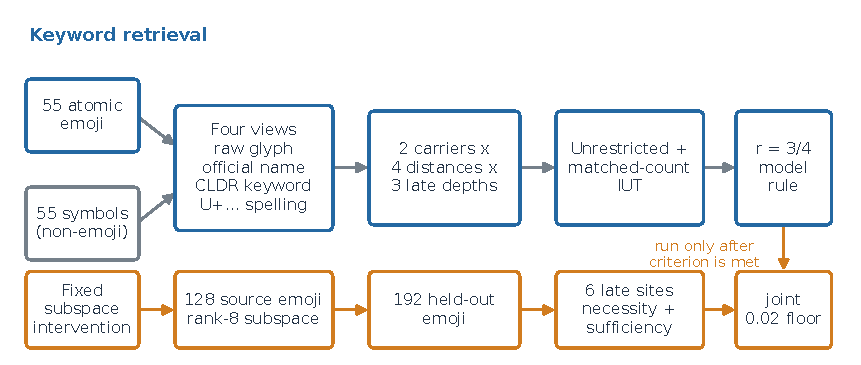
\includegraphics[width=\linewidth]{figures/t19_design.pdf}
  \caption{Keyword retrieval and fixed-subspace intervention. Retrieval crosses two glyph kinds with four
  text views. Only the emoji endpoint enters the registered cross-model
  primary. Fixed-subspace intervention runs only after that criterion is met
  and uses disjoint source and evaluation emoji. No causal-set item receives
  an observational retrieval evaluation.}
  \label{fig:design}
\end{figure}

\subsection{Observational readout}

For each item and view, the prespecified evaluation pipeline appends one of two suffix carriers
(\texttt{" a"} or \texttt{" |"}) at distances 1, 2, 4, and 8 and records the
hidden state at the selected suffix token at nine normalized depths. Batch
size is one; no chat template or added special token is used. The primary
late window is fixed at depths $0.75$, $0.875$, and $1.0$, yielding 24
contexts per item.

\paragraph{Running example: input, position, and score.}
For U+1F923, the four inputs begin with the raw Unicode character, the words
\texttt{rolling on the floor laughing}, the keyword \texttt{lmao}, or the
ASCII string \texttt{U+1F923}. In the pipe context each is followed by eight
copies of \texttt{ |}. Distance 1 reads the first suffix token's hidden
state; distance 8 reads the eighth. The tokenizer may split the raw character
into several tokens, together called the glyph positions. The model is never
asked to generate \texttt{lmao}; its readout vector is compared with all
keyword vectors in the gallery, including the matching item. This example illustrates the procedure
and makes no claim about that individual item's result.

\paragraph{Depth selection.}
The three late depths were inherited from the preceding study before the
present acquisition. The rule $\min(L-1,\lfloor fL\rfloor)$ maps normalized
depth $f$ to a zero-based block index in a model with $L$ blocks. For the
28-block Llama checkpoint, it yields blocks 21, 24, and 27. These are
prespecified sampling locations; they have no established status as universal
semantic stages. Appendix \ref{app:sensitivity} reports sensitivity to the
late-window average using saved observational summaries.

Within each view and context, hidden states are centered across items and
row-L2-normalized; $z^{v,c}_i$ denotes the vector for item $i$, view $v$, and
context $c$. Cross-view top-1 retrieval is

\begin{equation}
  R_c(g \rightarrow v) = \frac{1}{n}\sum_{i=1}^{n}
  \mathbf{1}\left[i = \arg\max_j
  \left\langle z^{g,c}_i, z^{v,c}_j \right\rangle\right].
  \label{eq:retrieval}
\end{equation}

The per-model primary estimate is

\begin{equation}
  \Delta_m = \frac{1}{24}\sum_c
  \left[R_c(g \rightarrow \alias) -
  R_c(g \rightarrow \codepoint)\right]
  \label{eq:primary}
\end{equation}

on the 55 observational emoji. This score measures nearest-neighbor retrieval
from hidden states.

\subsection{Token-count intersection and cross-model test}

Every model must pass two components. The unrestricted component uses all 55
emoji and permutes keyword correspondence within glyph kind. The matched
component retains non-singleton strata sharing the exact four-view
token-count signature and permutes keywords only within stratum. Retrieval in
that component uses the retained pool ($n=31$--$51$ emoji across models).
Uniform guessing over this gallery has rate $1/n$; the within-stratum
randomization expectation depends on stratum membership of the predictions.
Unrestricted and matched magnitudes are not directly commensurable.
Matching compares the four-count tuple across items. It does not require the
four views of one item to have equal token counts.
Official-name and codepoint correspondences stay fixed.
Thus the one-sided randomization test asks whether the fixed keyword mapping
beats mappings allowed by its null; because the codepoint term is fixed, it is
not a paired significance test of keyword--codepoint equality. The registered
primary combines that test with the observed comparative requirement
$\Delta_m\geq0.02$ in both components.
The 0.02 floor is a prespecified operational requirement of two percentage
points. It has no independent calibration to human meaning or practical
utility. Appendix \ref{app:sensitivity} therefore reports descriptive
threshold sensitivity while preserving the original decision.
Each component uses 19,999 draws, and the model intersection--union test
(IUT) $p$-value is the maximum of the two component values.

The sole cross-model primary uses four prespecified core configurations: Llama 3.2 3B base,
Qwen2.5 7B base, OLMo 2 1B base, and Gemma 2 2B IT. It tests the partial
conjunction that at least $r=3$ of $m=4$ configurations pass
\citep{benjamini2008partial}. With ordered model IUT values
$p_{(1)}\leq\cdots\leq p_{(4)}$, the registered value is
$p_{\mathrm{PC}}=\min(1,2p_{(3)})$. The other five configurations and all symbol or
official-name results are secondary and cannot admit the causal arm.

For keyword retrieval, percentile intervals from 20,000 item-bootstrap
replicates describe uncertainty; its primary decision uses the randomization
tests above. The subsequent causal designs also use bootstrap lower bounds
in their prespecified decision rules.

\subsection{Fixed-subspace intervention}

After the observational criterion was committed, fixed-subspace intervention ran in the
prespecified Llama 3.2 3B base configuration. The six sites are the attention
and MLP component outputs at blocks 21, 24, and 27: the tensors returned by
the attention output projection and by the MLP down-projection, hooked before
their residual addition. At each site we learned a rank-8 basis from the left
singular directions of the centered, row-normalized glyph--keyword
cross-covariance on 128 source emoji. The control basis is constructed
deterministically: sixteen seeded Gaussian directions inside the source
span are deflated against the learned basis and orthonormalized, and the
first eight are kept. Blocks 24 attention and MLP were primary; blocks 21
and 27 were secondary.
Block 24 was specified in advance; the protocol supplies no separate
empirical calibration establishing it as the uniquely appropriate primary site.

On 192 different evaluation emoji, the two criteria intervene on different
forwards. Necessity intervenes on the glyph forward: with $P$ the learned
rank-8 projector and $\mu$ the source-set glyph mean at the site, the site
output $g$ is replaced by $g-P(g-\mu)$. Sufficiency intervenes on the
codepoint forward: the site output $c$ is replaced by $c+P(g-c)$, using the
same item's glyph forward, with the replacement cast to BF16 at injection.
Analogous operations in the random basis define adjusted effects:

\begin{align}
N_s &= E_s(\text{random removal})-E_s(\text{learned removal}),\\
S_s &= E_s(\text{learned patch})-E_s(\text{random patch}).
\end{align}

Both source and evaluation inputs append eight copies of the single-token
\texttt{" |"} suffix; the intervention and readout use its first token
(distance 1). The endpoint reads the final hidden state of the intervened
forward at that token as a query against two fixed 192-row galleries built
once from clean, un-intervened forwards: the keyword states and the codepoint
states. Query matrix and each gallery are independently centered by their own
item means, row-normalized, and scored by cosine top-1 identity, giving
$E_s=$ keyword top-1 minus codepoint top-1. The glyph query measures the
baseline and necessity conditions. The patched codepoint query measures
sufficiency; there the codepoint term is self-retrieval and equals 1 at
baseline, so a patch can raise $E_s$ either by real keyword gains or by
destroying self-retrieval, and Section \ref{sec:results} reports the two
components separately. $E_s$ shares the item-wise contrast definition with
keyword retrieval while using a different item pool and one fixed context. A site must
have both adjusted effects and both lower 95\%
item-bootstrap bounds above $0.02$, pass both one-sided sign-flip tests
(99,999 draws), pass zero-hook and remove-restore engineering controls, and
survive Holm correction across the two primary sites
\citep{holm1979sequential}. No site, rank, depth, carrier, subset, or endpoint
was replaced after observing the result.
Here, \emph{fixed} means that the source-learned basis is held constant during
evaluation. In the next experiment, \emph{optimized} denotes interchange
training of the basis; it supplies no guarantee of an optimal explanation.

\subsection{Optimized-subspace intervention}
\label{sec:t20}

The fixed-subspace design left its own power uncalibrated. A second experiment,
specified after that analysis was validated and recorded, makes
five prespecified changes. (i) The rank-8 basis is learned by optimization:
an orthogonally parametrized subspace is trained on the same 128 source emoji
by interchange optimization (InfoNCE toward the own-item keyword state for
the patched codepoint forward, plus a hinge pushing the ablated glyph forward
below its own keyword), with a fixed 96/32 train/validation split, three
seeds, and a fixed selection rule; the closed-form and random bases are
recomputed at every site as comparators. (ii) The residual stream after
blocks 21, 24, and 27 joins the six component sites, with the block-21 and
block-24 residual sites primary. (iii) The decision uses the keyword
component alone, with a codepoint self-retrieval guard ($\geq0.90$ under the
learned patch), so disruption cannot pass as sufficiency. (iv) Evaluation
uses 384 atomic emoji with zero prior forwards in these experiments. The original
selection had to be reproduced byte for byte before these items were drawn.
Each item is read in four contexts (two carriers $\times$ distances 1 and 4),
and its scores are averaged across contexts. (v) Every site has two
full-state reference swaps: the entire
site state is exchanged between same-item glyph and codepoint forwards. By
the registered rule, a primary site that fails while its full-swap sufficiency effect
is below $0.06$ is recorded as \emph{uncalibratable at this endpoint}.
This verdict leaves the low-rank account unresolved; the control cannot turn
a failed decision positive. Floors, tests, Holm correction, and exact
engineering checks are unchanged from fixed-subspace intervention.
The historical protocol calls these swaps \emph{ceilings}; no universal
upper-bound property is established.

\subsection{Attention-path intervention after readout reset}
\label{sec:t21}

A pilot on the 384 already evaluated optimized-subspace items selected block 21 from
blocks 21/24 under a specified screening rule. Before accessing the remaining
195 unused evaluation emoji, we specified a new test. After replacing the
readout residual with its codepoint-view state, blocks 22--27 receive
token-count-matched donor keys and values at glyph positions, solely for the
readout query. Equal-count suffix replacement and full-prefix replacement
with glyph/suffix restoration provide controls. The endpoint is own-keyword
cosine similarity minus the largest similarity to 128 fixed source keywords,
referenced to the same batch slot with path replacement disabled. Two donors
and two carriers at distance 8 are averaged within each item. Five
calibration/decrement/restoration contrasts must have positive simultaneous
one-sided 95\% item-bootstrap lower bounds (20,000 draws). Appendix
\ref{app:t21} gives the exact contrasts, prospective order, and secondary
top-1 measures.

\paragraph{Prospective specification and execution checks.}
\label{sec:freeze}

Before acquisition, checksum records bind the protocol, code, and item sets
with evaluation forward counts still zero. Each causal arm links its
specification to the preceding validated analysis and requires publication
to the repository's default branch. Each invocation rejects changed code or
inputs. Dated specifications, admission records, execution manifests, and
independent validation reports in the supplement preserve the order of
specification, conditional admission, and evaluation.
These are timestamped internal prospective specifications, not registrations
in an external registry.

\section{Results}
\label{sec:results}

\subsection{A lexical relation beyond the official short name}

The registered cross-model primary passed. All four core configurations were positive;
the third-smallest core IUT value was $0.00135$, yielding
$p_{\mathrm{PC}}=2(0.00135)=0.0027$. All nine prespecified configurations were positive and
exceeded the registered $0.02$ effect-size floor in both unrestricted and matched analyses
(Figure \ref{fig:model-effects}; exact values in Appendix
\ref{app:observational}). Model IUT values ranged from $0.00005$ to $0.00185$.
The smallest unrestricted effect, Qwen2.5 0.5B at $+0.03636$, equals an
average margin of two net top-1 matches per 55-item context. A validator that
does not import the acquisition analyzer reconstructed all 36 randomization
tests and reproduced the primary decision.

\begin{figure}[t]
  \centering
  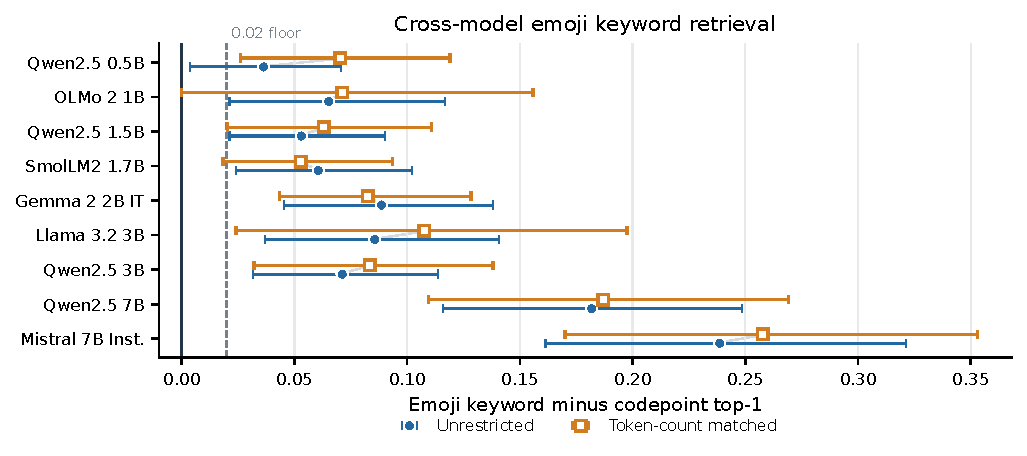
\includegraphics[width=\linewidth]{figures/t19_model_effects.pdf}
  \caption{Emoji keyword-minus-codepoint top-1 effects in the registered roster
  order. Bars are descriptive 95\% item-bootstrap intervals (20,000
  replicates); randomization tests determine the primary decision. The
  $0.02$ floor applies to point estimates. Unrestricted (U) and matched (M)
  analyses use different retained pools, so their magnitudes are not directly
  commensurable. Every displayed point estimate exceeds the floor.}
  \label{fig:model-effects}
\end{figure}

Across models, mean emoji keyword effects were $+0.0979$ unrestricted and
$+0.1084$ matched. Mean official-name effects were larger, $+0.1440$ and
$+0.1718$. Thus, retrieval extends beyond the exact official name, although
the official name remains the stronger key on average. The alternative label
is an exact CLDR keyword, not a human-rated synonym or paraphrase;
training-data co-occurrence could still fully explain the relation.
Descriptively, the unrestricted effect also rises monotonically with
parameter count inside the one family sampled at four sizes (Qwen2.5:
$+0.036$, $+0.053$, $+0.071$, $+0.182$ from 0.5B to 7B). The roster remains
confounded across families, so this ordering is description, not a registered
scale result.

Depth was secondary. Across models and contexts, the unrestricted contrast
was $+0.0409$ at depth 0 and $+0.0864$, $+0.1152$, $+0.0922$ at the three
primary depths, whose mean is the $+0.0979$ above; onset and peak depths
differed across configurations, so these data do not support one universal
trajectory.

Post-outcome arithmetic on the saved estimates retains all nine configurations
when the point-estimate floor is raised to $0.03$. Each of the three late
depths alone also retains all nine above $0.02$. These sensitivity checks
leave the original test unchanged and supply no new depth-specific $p$-values
(Appendix \ref{app:sensitivity}).

\subsection{A named-symbol control limits the emoji-specific claim}

Non-emoji symbols showed mean keyword effects of $+0.0236$ unrestricted and
$+0.0153$ matched, compared with $+0.0979$ and $+0.1084$ for emoji. The
emoji-minus-symbol point estimate was positive in all nine configurations in both
components. Symbol keywords were heterogeneous: Qwen2.5 3B and 7B were
negative in both components. Official-name retrieval exceeded keyword retrieval
for symbols in 9/9 configurations in both components, with mean symbol official-name effects
of $+0.0750$ and $+0.0821$ (Figure \ref{fig:symbol-boundary}).

This comparison cannot establish an emoji-specific faculty: the panels are
not matched on training frequency, lexical specificity, Unicode category,
visual familiarity, or token identity. Its role is to prevent the incorrect
inference that only emoji acquire readable names.

\subsection{No prespecified late-component site passes both causal criteria}

Before intervention, the final-hidden glyph endpoint on the 192-item causal
evaluation set was $E_s=0.07292$ (keyword top-1 $0.07292$, i.e.\ 14 of 192
items; codepoint top-1 $0$); the zero-hook engineering check reproduced this
baseline identically at all six sites. This is the glyph-input baseline used
by the necessity arm; the sufficiency arm starts from codepoint inputs, whose
keyword top-1 is $1/192$ and whose codepoint term is self-retrieval at
$192/192$. The
$0.02$ decision floor was therefore 27\% of this baseline contrast, and the
design contained no positive intervention control that calibrated attainable
adjusted necessity at the primary sites. All six causal sites passed
their engineering checks: zero-hook and
remove-restore conditions reproduced the baseline final hidden state with
exactly zero RMS difference. Bitwise equality is expected because baseline
forwards reuse the exact intervention batch geometry; any nonzero residue
would indicate an instrumentation or batching mismatch. Neither primary block-24 site
passed. Block-24 attention had adjusted necessity $0.0000$ and sufficiency
$-0.00521$; block-24 MLP had $+0.00521$ and $0.0000$. Their site IUT values
were $1.0$ and $0.74912$, respectively. None of the six sites passed both
components (Figure \ref{fig:causal}, Appendix \ref{app:causal}; exact values
in Table \ref{tab:causal}).

The secondary block-27 MLP patch produced adjusted sufficiency $+0.07812$.
Its 95\% interval was $[+0.03646,+0.11979]$, with one-sided $p=0.00009$
(uncorrected; twelve such component tests were run in total). Necessity was $-0.01562$ (interval
$[-0.04167,+0.00521]$, $p=0.96895$), giving a site IUT of $0.96895$.
The learned patch raised keyword top-1 from $1/192$ to $4/192$ while lowering
codepoint self-retrieval from $192/192$ to $180/192$. The keyword gain accounts
for 3 of the composite endpoint's 15 additional correct contrasts; the
remaining 12 arise from lost codepoint self-retrieval. This pattern is
consistent with broad representational disruption and does not identify a
necessary keyword mechanism.

A post-hoc calibration, computed after the registered decision and labeled as
such, replaced the entire component output with the same item's other-view
output at each site (Appendix \ref{app:causal}). Full interchange at the
primary block-24 sites moved keyword top-1 by $0.0000$ (attention) and
$+0.0052$ (MLP). These complete replacements fell below the $0.02$ floor,
limiting what the primary negative can establish about rank. The block-27
MLP full-swap composite effect ($+0.2448$ against a
keyword-only $+0.0365$) quantifies how much of that endpoint's headroom was
destroyed self-retrieval. These numbers motivated the full-state controls of
the follow-up.

\subsection{Full-state controls reveal a depth-dependent asymmetry}
\label{sec:t20-results}

Both primary optimized-subspace residual sites return the registered verdict
\emph{uncalibratable at this
endpoint} (site IUT values $0.624$ and $0.679$; full-swap sufficiency effects
$+0.0234$ and $+0.0254$, below the registered $0.06$ minimum). No secondary
site passes either. All engineering checks are again exactly zero, and an
independent validator re-derived every reported number, both verdicts, and
the admission chain.

The registered full-state controls reveal a depth-dependent pattern
(Figure \ref{fig:t20-ceilings}; exact values in Appendix \ref{app:t20}). On
the new evaluation set, glyph-input keyword top-1 is $0.0345$ and
codepoint-input top-1 is $0.0013$, a baseline gap of $0.0332$. Swapping the
readout-token residual stream at block 27 reproduces both baseline retrieval
rates exactly, as expected because the endpoint is a function of that state.
At blocks 21 and 24, injection transfers $71\%$ and $76\%$ of
this gap; replacement in the glyph forward removes only $4\%$ and $25\%$.
Retrieval therefore remains near baseline after the readout-token stream is
replaced at these earlier sites. Component-output swap effects at blocks 21
and 24 are smaller (at most $14\%$ of the gap; block-24 attention sufficiency $2\%$).
This asymmetry motivated the attention-path test of later glyph-position messages.

Training trajectories improve with limited held-out benefit; Appendix
\ref{app:t20} reports the training, validation, and self-retrieval diagnostics.

\begin{figure}[t]
  \centering
  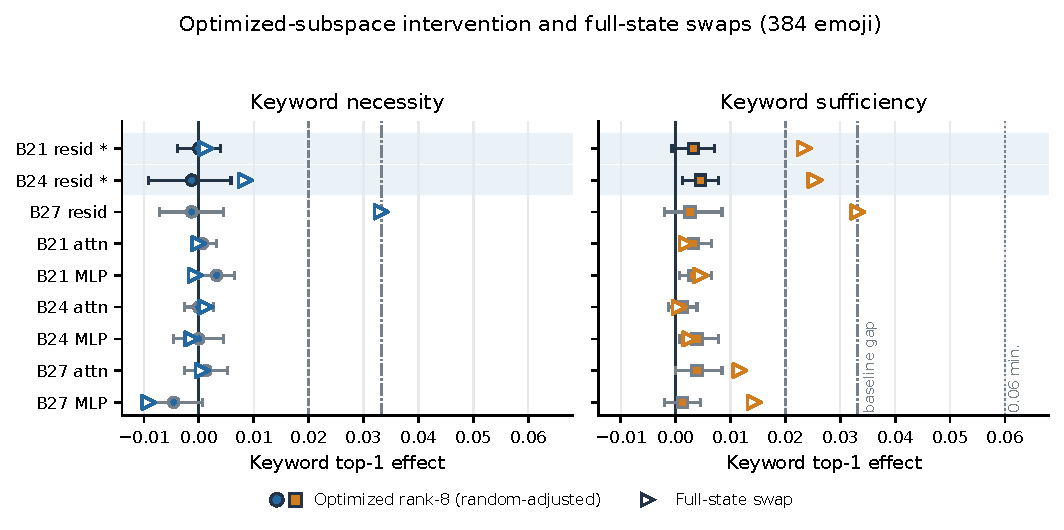
\includegraphics[width=\linewidth]{figures/t20_causal_ceilings.pdf}
  \caption{Optimized-subspace intervention on 384 evaluation emoji in four contexts.
  Filled markers show random-adjusted rank-8 optimized effects with
  descriptive 95\% item-bootstrap intervals; open triangles show the
  full-state reference swaps at the same sites. Shaded rows mark the two
  primary residual sites; the dashed line is the registered $0.02$ floor and
  the dotted line the $0.06$ reference-effect minimum. The
  block-27 residual swap is an expected endpoint-consistency check (the
  dash-dotted line marks the $0.0332$ baseline gap). Neither primary sufficiency
  reference effect clears $0.06$, so both sites are uncalibratable under the registered rule.}
  \label{fig:t20-ceilings}
\end{figure}

\subsection{A conditional attention-message contribution}
On all 195 attention-path evaluation items, the five simultaneous lower bounds are positive.
Glyph-message decrement exceeds the suffix control by $0.002326$ in cosine
margin (lower bound $0.001399$), and restoration exceeds its control by
$0.002267$ (lower bound $0.001400$; Figure \ref{fig:t21-path}). Both carriers have
positive means separately. Absolute glyph-message decrement and restoration
each have zero mean keyword top-1 effects. Post-reset baseline accuracy is
low (pipe $3.08\%$; article carrier $0.51\%$). The positive result concerns
relative similarity. Independent CPU reconstruction agrees on every metric,
bound, and the prespecified verdict.
A post-hoc decomposition finds positive own-keyword shifts in both adjusted
means, partly offset by increased competitor similarity (Table
\ref{tab:t21-decomposition}).

\begin{figure}[t]
  \centering
  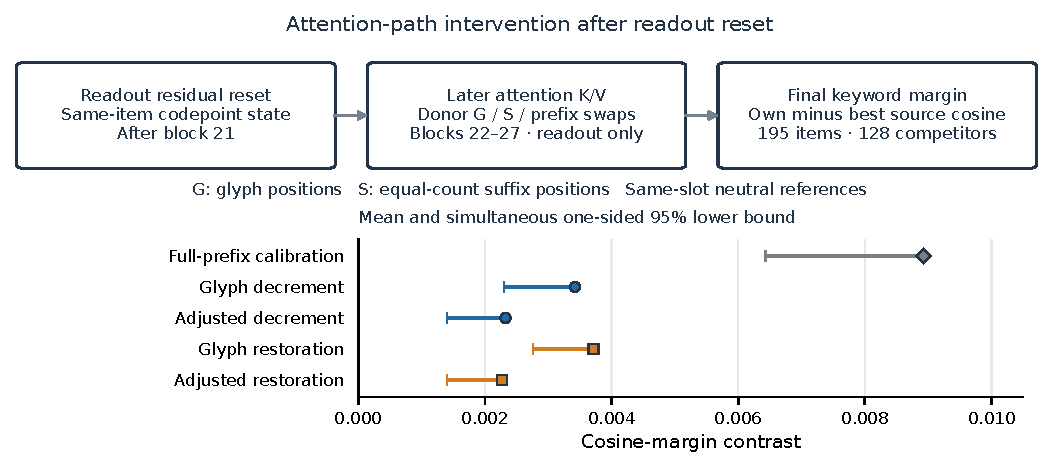
\includegraphics[width=\linewidth]{figures/t21_path_summary.pdf}
  \caption{Attention-path intervention after readout reset: five margin contrasts.
  A 384-item pilot selected block 21 before the 195-item confirmation.
  Points are means; each segment joins its simultaneous one-sided 95\%
  lower bound to the mean (20,000 shared-index item-bootstrap draws).
  All five lower bounds exceed zero. Effects average two carriers and two
  fixed-pool donors within each item; absolute top-1 decrement and restoration
  have zero mean effects. Table \ref{tab:t21} gives exact values.}
  \label{fig:t21-path}
\end{figure}

\section{Discussion}

Keyword retrieval establishes a word-disjoint lexical relation after token-count matching.
Fixed and optimized subspace interventions constrain the tested rank-8 accounts
within their calibration limits. Retrieval preserved after earlier readout-state replacement
suggested later use of the unchanged prefix. Attention-path intervention confirms a conditional
glyph-position margin contribution on new items after a readout reset.
Its different population and endpoint leave the
full explanation of the optimized study's swap asymmetry open.

State replacement and pathway intervention answer distinct causal
questions. Endpoint decomposition clarifies the results: the fixed-subspace block-27 MLP patch
chiefly degrades codepoint self-retrieval; the path intervention shifts both own-keyword and
competitor cosines, yielding positive adjusted margins with zero mean absolute
top-1 effects.

\subsection{Development extension: measuring contextual responses}
\label{sec:development}

Following the lexical experiments, we examined teacher-forced response
probabilities in 24 authored scenarios from six recurring families. Two goal
contexts were crossed with emoji and word cues, using three continuation
formulations. The matched-execution scoring version retains positive
context--cue interaction across every formulation in 22/24 emoji and 23/24
word scenarios. Absolute candidate preference changes across formulations
on 55/96 emoji and 56/96 word inputs. Neither carrier has a scenario with
author-aligned choices in all four inputs across every formulation. A stable
cue meaning combined with a changing goal can generate such interactions.

A subsequent development design separated property matching, message
interpretation, and evidence that an outcome occurred. One previously exposed
author supplied 36 judgments on 24 scenes: 26 were binary and ten undecidable.
Same-question model agreement was 16/26 on the binary subset; all 36 selected
model choices also follow a post-hoc question-type constant rule. Across the
full model inventory, 710/816 true/false wording pairs imply inconsistent
truth, and all 48 positive-worded accurate-completion controls prefer No.
These limitations concern the tested Llama 3.2 3B base checkpoint and its
prompt/readout configuration. Exact numerical replay alone cannot qualify
this format as a measure of contextual interpretation.

Appendix~\ref{app:contextual} records the complete developmental comparison,
including adverse controls and a token-level sensitivity analysis. The same
scenarios are reused throughout, with no new confirmatory sample or population
inference. A subsequent, prospectively specified qualification uses 32 new
text-only facts in four authored families, with explicit-positive,
explicit-negative, and unknown reports (Appendix~\ref{app:qualification}).
Direct questions with minimal Yes/No answers are correct on 88/96 reserved
cases, with four errors and four ties; eight of 16 roots satisfy all six
conditions. Full-sentence answers score 75/96 on the same direct questions,
and minimal answers score 65/96 and 57/96 under nested-true and nested-false
questions. The primary fails its specified 96/96 requirement; explicit A/B
remappings separately fail at 104/192, with 19 ties. These controlled text-only
comparisons identify question and encoding dependence before any emoji
interpretation is required. Independent assessment and an output measure
qualified for its intended task remain prerequisites for a natural-state
causal study. The earlier conditional attention result establishes no such
output connection.

\section{Limitations and broader impact}

\paragraph{Measurement.}
CLDR keywords were not human-rated for synonymy, specificity, or familiarity.
Retrieval measures
nearest-neighbor geometry at selected suffix tokens. Free generation,
validated task performance, and rendered-glyph perception were not tested. Token-count matching
leaves token identities and tokenizer construction uncontrolled.
Low post-reset top-1 baselines may limit detection of decrements; zero means establish
neither equivalence nor unchanged outcomes for every item.

The response extension is unfinished instrument development on reused,
author-written scenarios. Repeated formulations and six scenario families
constrain independence. Word and emoji cues differ in explicitness and
token/position geometry. The single author knew prior project results;
the tryout supplies no independent semantic labels. Human uncertainty and
forced model choices have different response spaces. Track revisions also
change some constructs, including visible expression versus affect, so they
do not isolate an instruction-only effect. The controls qualify neither
semantic accuracy nor a general failure of the model to understand negation.
The later 32-root qualification is a finite, source-authored check, with repeated
report and question conditions and a deliberately strict all-cases-correct
requirement. Its four primary errors coexist with four ties under the fixed
BF16 computation; no precision comparison identifies their cause. It adds
no human semantic labels or model-population estimate.

\paragraph{Generalization.}
The nine model--tokenizer configurations form a prespecified convenience roster
spanning several families and sizes \citep{yang2024qwen25,olmo2024furious,
dubey2024llama3,gemmateam2024gemma2,jiang2023mistral,benallal2025smollm2}.
Family, size, training data, tokenizer, and instruction tuning are confounded;
scale laws and model-population estimates remain unsupported. Emoji surfaces
may have appeared in pretraining; the symbol-panel
freshness criterion concerns only repository history.

\paragraph{Mechanism.}
Mechanistic tests cover one Llama 3.2 3B checkpoint. The two subspace studies use rank-8,
single-site readout-token interventions; the path test conditions on a codepoint-view
reset, two carriers, and a fixed donor/gallery pool. Suffix controls match
position count alone; attention mass and semantic content remain uncontrolled.
Non-emoji path controls, separate key/value effects, sparse feature bases
\citep{bricken2023monosemanticity,cunningham2024sparse}, and nonlinear readouts
remain untested. Path-test item-bootstrap coverage is approximate and limited to the
eligibility-defined population. Fixed-subspace intervention lacked a positive intervention control;
optimized-subspace intervention specified full-state swaps \citep{geiger2024das,wu2023boundless}
and returned uncalibratable primary verdicts. These reference swaps have no
proven universal upper-bound property. Training on 96 items leaves item-specific
coding, limited data, and optimization as explanations for weak generalization.
The 384-item baseline gap ($0.0332$) falls below the $0.06$ threshold chosen
from the smaller fixed-subspace set. Future thresholds should be calibrated on a
separate development set before specifying evaluation.

\paragraph{Reproducibility and impact.}
The anonymous compact archive binds configurations, selections, summaries,
tests, validators, licenses, and the September manuscript; raw arrays remain in the execution
environment. Exact retrieval/fixed-subspace acquisition duration and peak memory are absent from
the submitted evidence. Unicode auditing could reveal representation failures
in multilingual systems. Applying CLDR correspondence to people's meaning,
sentiment, culture, or identity risks unjustified profiling. The historical
lexical and intervention experiments use no human responses or private messages.
The development extension adds an author-only tryout. Its individual responses,
assignments, and notes remain private; this local draft includes aggregates
only. No external participants were recruited. Formal approval or exemption
for future human evaluation is not claimed, and its review and release
arrangements remain to be specified.

\section{Conclusion}

Across nine prespecified model--tokenizer configurations, raw atomic emoji
retrieve word-disjoint CLDR keywords better than literal codepoints after
exact four-view token-count matching. A named-symbol control bounds the
specificity of this result. Two separately partitioned causal
experiments leave the tested rank-8 readout-token account unsupported.
A separately specified 195-item follow-up confirms a conditional glyph-position
attention contribution to keyword margin, with zero mean absolute top-1
effects. Together, these experiments separate recoverable lexical information
from the conclusions licensed by each intervention. Subsequent contextual
response scoring finds interactions alongside substantial formulation and
polarity dependence. A new explicit-report qualification records partial
success on simple facts alongside failures of the specified primary and
label-robustness criteria. Together, these results identify measurement
limits that precede interpreting response scores as meaning judgments.
Independent validation, free generation, and output-linked causality remain
open.\label{sec:main-end}

\clearpage
\bibliographystyle{plainnat}
\bibliography{references}

\clearpage
\appendix

\section{Exploration path and decision lineage}
\label{app:lineage}

Historical identifiers map to the reader-facing names as follows:
T19-L is \emph{keyword retrieval}; T19-C is \emph{fixed-subspace intervention};
T20-C is \emph{optimized-subspace intervention}; and T21-C is
\emph{attention-path intervention after readout reset}.
T19-L was the observational arm of the nineteenth study in this project.
The concise lineage below includes only results that changed the next design
decision. Earlier studies retain their exploratory or failed-confirmation
status; the T19-L primary uses its own prespecified evidence alone.

Figure \ref{fig:lineage} groups the sequence by the question each stage
addressed. The labels trace how the design changed.

\begin{figure}[t]
  \centering
  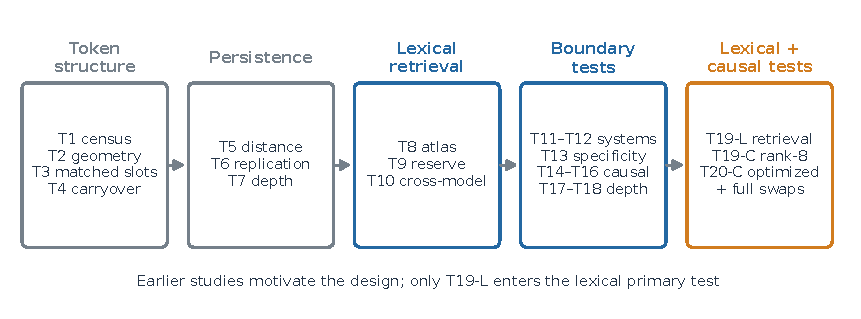
\includegraphics[width=\linewidth]{figures/t19_lineage.pdf}
  \caption{Exploration-to-confirmation lineage. Early studies exposed
  token-structure and persistence explanations; later studies narrowed the
  endpoint and causal test. Arrows record design decisions, not evidence
  pooling. Only the T19-L primary supports the confirmatory lexical claim in
  this paper.}
  \label{fig:lineage}
\end{figure}

\paragraph{Initial screen and matched controls (baseline and Milestone 2).}
An initial colored-shape screen produced 25 positive results among 36
layer--seed--dose configurations. An exact tokenization-matched follow-up
supported one tested layer contrast and failed to support the other. We made
tokenization part of the estimand, retained negative configurations, and
stopped treating a pooled steering score as one stable semantic effect.

\paragraph{Token structure and short-range carryover (T1--T4).}
T1, the \emph{multifamily tokenizer census}, found no universal token-count
and prefix match for the fixed colored-shape panel. T2, \emph{multifamily
colored-shape geometry}, yielded no dual-model recurrence at the selected
midpoint. T3, \emph{five-family matched-slot geometry}, found recurrence only
in OLMo, where the exact shared slot token was already a sufficient
explanation. T4, \emph{common-suffix carryover}, showed that the OLMo pattern
persisted one common token later. The sequence converted tokenizer structure
from a nuisance variable into an explicit competing explanation.

\paragraph{Persistence, depth, and the lexical turn (T5--T8).}
T5, the \emph{carrier-distance profile}, and T6, the \emph{dense CUDA
carrier-distance replication}, both failed their prespecified
distance-attenuation conjunctions. T7, \emph{Mistral base
depth-by-distance}, passed an early-versus-late interaction in a model and
endpoint selected after T6, so it remained prospective within that configuration
rather than independent confirmation. T8, the \emph{Mistral semantic atlas},
then mapped 842 discovery emoji and found a large descriptive
name-over-codepoint contrast. That atlas supplied the endpoint later tested on
the untouched T9 reserve.

\paragraph{Lexical exploration and failed reserves (T9--T12).}
A held-out Mistral configuration first supported name-over-codepoint retrieval. A
nine-configuration follow-up retained statistical signal and failed its
registered cross-model effect-size rule. Broader glyph-system exploration then suggested
Unicode-composition hypotheses; neither survived testing on separately
reserved items. We kept both failures, dropped the generic composition claim,
and returned to a narrower lexical question.

\paragraph{Specificity decomposition and first causal localization (T13--T14).}
T13 separated structured source directions from generic target susceptibility
on already exposed panels and remained exploratory. T14 then paired a signed
six-model intervention grid with a separately specified selected-site test.
The broad response pattern was heterogeneous across model, depth, source form,
null family, and sign; the selected Llama component failed the joint causal
criterion on a new evaluation set. This combination motivated the
response-shape tests and stricter causal separation in T15--T16.

\paragraph{Readable responses and unsuccessful causal tests (T15--T16).}
An emoji--word response pattern replicated prospectively, and prespecified
forced-choice associations were detectable. Yet a subspace intervention and
a multi-layer transplantation each failed their stronger causal criteria. This
separated readout from implementation and motivated the present joint
necessity--sufficiency criterion.

\paragraph{Depth mapping and fresh confirmation (T17--T18).}
Across 292 previously exposed atomic emoji, name-minus-codepoint retrieval was
positive in all nine model configurations at middle-to-late depths. Peaks were
model-specific, and final item retrieval (9/9) did not require consistent
whole-representation CKA alignment (4/9 configurations). We therefore
prespecified a common late window, replaced the population, and made no shared-transition or
universal-manifold claim. On 192 repository-fresh composite emoji, the
official-name contrast then
passed in 4/4 core configurations and 8/9 configurations overall after exact token-count
matching. This justified asking whether the relation extends beyond the
official short name, while adding a named non-emoji control and reserving new
item sets for causality. This T18 composite set is distinct from the 192
atomic emoji in the T19-C evaluation set.

\paragraph{T19-L and T19-C (confirmatory and first conditional arm).}
T19-L replaces the sole label endpoint with a word-disjoint CLDR keyword and
adds literal-codepoint and named-symbol boundaries. T19-C tests the prespecified
rank-8 component account on disjoint source and evaluation sets. Broad
lexical retrieval passes, while the simple late-component mediator fails its
joint criterion.

\paragraph{T20-C (second conditional arm).}
The T19-C result, recorded without a positive control, motivated a separate
prespecified experiment. T20-C was specified and authorized after the T19-C
analysis was validated; its execution manifest identifies that analysis by
checksum. Its five changes (optimized subspaces, residual-stream sites,
keyword-only decision, a new 384-item four-context evaluation set, and
registered full-state controls) each address a T19-C limitation. The
registered verdict is uncalibratable at both primary sites. The measured
swap asymmetry motivates the pathway hypothesis in Section \ref{sec:t20-results}.

This lineage explains why the final design contains four text views, exact
token-count strata, a non-emoji symbol panel, three disjoint item sets, and a
necessity--sufficiency intersection. It also explains what is absent: no
favorable prior layer, glyph system, or causal site was promoted into the
T19-L primary. Only that prespecified primary supports the paper's confirmatory
lexical claim.

\paragraph{T21 (exposed-item pilot followed by a new confirmation).}
The T20-C swap asymmetry suggested a glyph-position attention route. A
384-item pilot reused the T20 evaluation items to choose between anchors
21/24; it contributed no new confirmatory items. A separate protocol then
specified the remaining 195 items, a cosine-margin endpoint, and a
five-contrast simultaneous rule before their reconstruction or evaluation.
The resulting conditional path contribution and zero mean absolute top-1
effects are reported in Appendix \ref{app:t21}; T19/T20 verdicts are retained.

\section{Prespecified examples and model roster}
\label{app:models}

\begin{table}[H]
\centering
\scriptsize
\setlength{\tabcolsep}{2.5pt}
\begin{tabular}{p{0.17\linewidth}p{0.35\linewidth}p{0.15\linewidth}p{0.20\linewidth}}
\toprule
Raw scalar$^\dagger$ & CLDR \texttt{tts} & Keyword & Literal view \\
\midrule
U+1F923 & rolling on the floor laughing & lmao & \texttt{U+1F923} \\
U+1F928 & face with raised eyebrow & skeptic & \texttt{U+1F928} \\
U+00B4  & acute accent & tone & \texttt{U+00B4} \\
\bottomrule
\end{tabular}
\caption{Concrete prespecified views for two emoji and one non-emoji symbol.
$^\dagger$The model receives the scalar itself; the table names it by codepoint
because the paper typeface need not render every glyph. The literal view is
the displayed ASCII string.}
\label{tab:examples}
\end{table}

Table \ref{tab:models} reports the exact model artifacts and revisions used by
the prespecified observational roster. The Llama BF16 mirror was retained
from initial development on Apple Silicon and specified in the protocol.
The reported runs loaded its safetensors through Transformers/CUDA.
The \texttt{mlx-community} identifier records artifact provenance; upstream
bit-identity was not verified. Model cards
and upstream license terms are part of the historical archive's license audit.
The cards declare Apache-2.0 for the Qwen2.5 0.5B, 1.5B, and 7B configurations, OLMo,
SmolLM2, and Mistral; Qwen2.5 3B uses the non-commercial Qwen Research
License, Gemma uses the Gemma Terms of Use, and the Llama mirror uses the
Llama 3.2 Community License. No checkpoint or tokenizer file is redistributed.

\begin{table}[H]
\centering
\scriptsize
\setlength{\tabcolsep}{3.5pt}
\begin{tabular}{lll}
\toprule
Role & Artifact identifier & Revision \\
\midrule
Qwen2.5 0.5B base & \texttt{Qwen/Qwen2.5-0.5B} & \texttt{060db6499f32} \\
OLMo 2 1B base & \texttt{allenai/OLMo-2-0425-1B} & \texttt{a1847dff3500} \\
Qwen2.5 1.5B base & \texttt{Qwen/Qwen2.5-1.5B} & \texttt{8faed761d45a} \\
SmolLM2 1.7B base & \texttt{HuggingFaceTB/SmolLM2-1.7B} & \texttt{effd688a1292} \\
Gemma 2 2B IT & \texttt{google/gemma-2-2b-it} & \texttt{299a8560bedf} \\
Llama 3.2 3B base & \texttt{mlx-community/Llama-3.2-3B-bf16} & \texttt{60a99aaf4316} \\
Qwen2.5 3B base & \texttt{Qwen/Qwen2.5-3B} & \texttt{3aab1f1954e9} \\
Qwen2.5 7B base & \texttt{Qwen/Qwen2.5-7B} & \texttt{d14972939875} \\
Mistral 7B Inst. v0.3 & \texttt{mistralai/Mistral-7B-Instruct-v0.3} & \texttt{c170c708c41d} \\
\bottomrule
\end{tabular}
\caption{Model artifact identifiers and the first 12 hexadecimal characters
of the exact revisions used. Full revisions are stored in the
submission manifest.}
\label{tab:models}
\end{table}

\section{Exact observational results}
\label{app:observational}

\begin{table}[H]
\centering
\small
\begin{tabular}{lrrrrc}
\toprule
Model configuration & M $n$ & U effect & M effect & Model IUT $p$ & Pass \\
\midrule
Qwen2.5 0.5B & 35 & 0.0364 & 0.0702 & 0.00055 & yes \\
OLMo 2 1B & 31 & 0.0652 & 0.0712 & 0.00135 & yes \\
Qwen2.5 1.5B & 35 & 0.0530 & 0.0631 & 0.00185 & yes \\
SmolLM2 1.7B & 41 & 0.0606 & 0.0528 & 0.00005 & yes \\
Gemma 2 2B IT & 51 & 0.0886 & 0.0825 & 0.00005 & yes \\
Llama 3.2 3B & 31 & 0.0856 & 0.1075 & 0.00135 & yes \\
Qwen2.5 3B & 35 & 0.0712 & 0.0833 & 0.00005 & yes \\
Qwen2.5 7B & 35 & 0.1818 & 0.1869 & 0.00005 & yes \\
Mistral 7B Inst. & 38 & 0.2386 & 0.2577 & 0.00005 & yes \\
\bottomrule
\end{tabular}
\caption{Exact reporting values for the registered emoji
keyword-minus-codepoint endpoint. U is unrestricted; M is exact four-view
token-count matched. The model IUT is the maximum component randomization
$p$-value.}
\label{tab:observational}
\end{table}

Matched emoji counts ranged from 31 to 51. The matched component retained at
least 63 observational items total in every configuration, with at least 31 emoji and
32 symbols; the unrestricted component used all 55 emoji and 55 symbols. The
acquisition comprised $9\times110\times4\times2=7{,}920$ batch-one forwards
(configurations $\times$ items $\times$ views $\times$ carriers). Four
distances and nine depths produced $7{,}920\times4\times9=285{,}120$ readout
vectors in 45 checksum-verified data files.

\paragraph{Conditional randomization benchmark and compact replay.}
For query $i$, let $s(i)$ be its exact token-count stratum and
$\hat\jmath_{i,c}$ its keyword prediction. The keyword hit rate expected under
the matched null is
\[
 \frac{1}{24n}\sum_{c,i}
 \frac{\mathbf{1}[\hat\jmath_{i,c}\in s(i)]}{|s(i)|}.
\]
This averages a fixed prediction's chance of matching its permuted label.
For Llama's 31-item matched emoji gallery it is $0.06650$; uniform guessing
over that gallery is $1/31=0.03226$. The codepoint term stays fixed. The
anonymous archive supplies all primary-window prediction indices and exact
strata for all nine configurations. A separate NumPy-only program reproduces
all 36 randomization tests, 36 descriptive intervals, model and Holm
decisions, and the cross-model $p=0.0027$ with zero numerical difference on
the acquisition platform. This is statistical replay from fixed predictions;
hidden-state reconstruction requires the retained arrays.

\subsection{Descriptive threshold and depth sensitivity}
\label{app:sensitivity}

The following checks were added during the October revision using five saved
compact result files, without new model forwards or randomization draws.
The supplied script \path{summarize_revision_sensitivity_v0.py} records
the SHA-256 of each input and reproduces the arithmetic. Historical protocols,
decisions, and statistical tests are unchanged.

\begin{table}[ht]
\centering
\small
\begin{tabular}{rrrc}
\toprule
Hypothetical floor & Both point estimates: all models & Core models & At least 3 of 4 core \\
\midrule
0.02 & 9/9 & 4/4 & yes \\
0.03 & 9/9 & 4/4 & yes \\
0.04 & 8/9 & 4/4 & yes \\
0.06 & 6/9 & 4/4 & yes \\
0.08 & 4/9 & 3/4 & yes \\
0.09 & 2/9 & 1/4 & no \\
\bottomrule
\end{tabular}
\caption{Post-outcome sensitivity of keyword retrieval to an observed-effect
floor. Both unrestricted and matched estimates must meet the floor. Stored
model tests are held fixed; the table reports no new inferential decisions.}
\label{tab:sensitivity}
\end{table}

The smallest of the two point estimates across all nine models is
$0.03636$; the third-largest core-model minimum is $0.08252$ (rounded).
The stored cross-model $p$-value remains $0.0027$ because the keyword
randomization tests are unchanged. A floor check and its permutation test
address different requirements of the original decision.

At normalized depths $0.75$, $0.875$, and $1.0$, the smallest point estimate
over models and unrestricted/matched components is respectively $0.02045$,
$0.05000$, and $0.03182$. Each leave-one-late-depth-out average also retains
all nine models above $0.02$. No primary $p$-value is transferred to these
alternative windows, and untested intervention depths remain unresolved.

For the six fixed-subspace and nine optimized-subspace sites, every saved
site has at least one nonpositive necessity/sufficiency lower bound and an
IUT $p$-value above $0.05$. Reducing their effect floor to zero would therefore
create no successful joint intervention. The optimized primary sites remain
uncalibratable under their original full-state reference rule. Changing that
rule afterward could change the label, not establish a successful intervention.

\begin{figure}[ht]
  \centering
  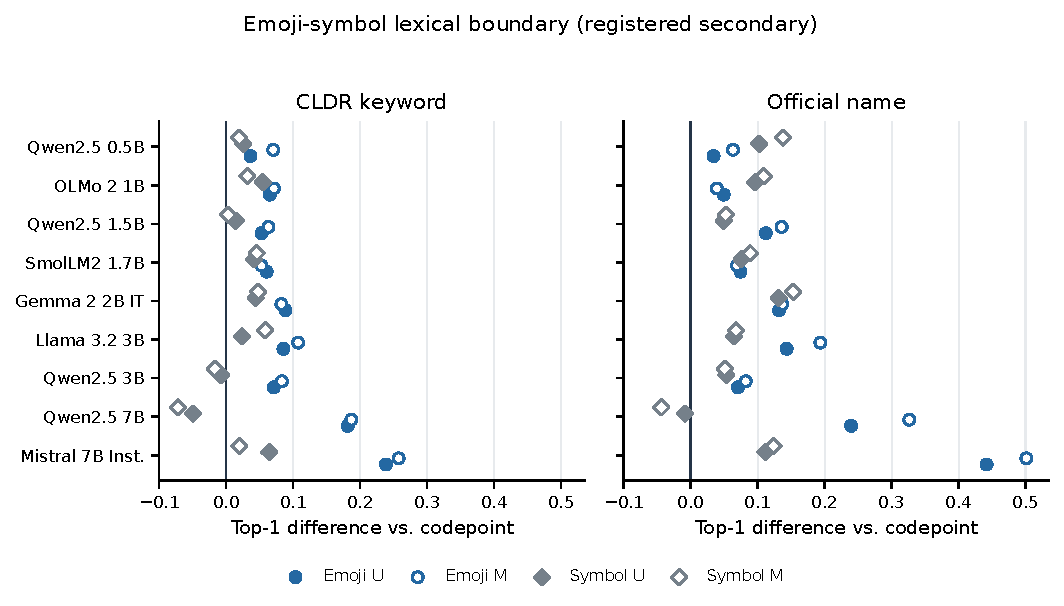
\includegraphics[width=\linewidth]{figures/t19_emoji_symbol_boundary.pdf}
  \caption{Registered secondary comparison. Each row shows unrestricted (U)
  and token-count-matched (M) effects for the same prespecified model.
  Official-name retrieval extends to non-emoji symbols; disjoint-keyword
  effects are stronger and more consistent for the prespecified emoji panel.
  Glyph category, frequency, label quality, and token identity are
  nonexchangeable across panels.}
  \label{fig:symbol-boundary}
\end{figure}

\section{Exact causal results}
\label{app:causal}

\begin{figure}[t]
  \centering
  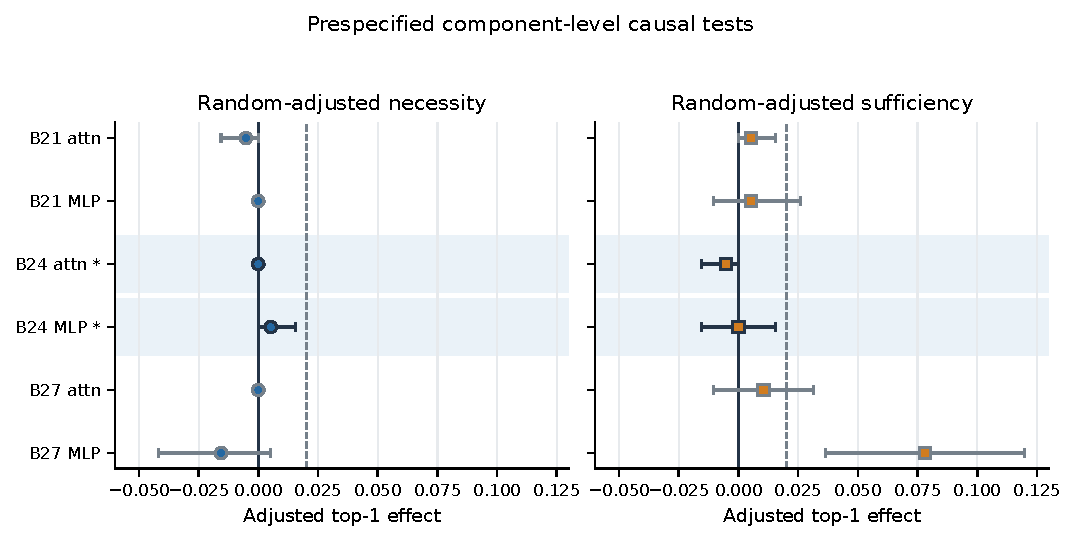
\includegraphics[width=\linewidth]{figures/t19_causal_sites.pdf}
\caption{Fixed-subspace intervention effects with descriptive 95\%
item-bootstrap intervals over 192 evaluation emoji. Shaded rows
  and asterisks mark the two primary block-24 sites. Solid vertical lines
  show zero; dashed lines show the registered $0.02$ effect-size floor. No
  site has both necessity and sufficiency above the floor with positive lower
  bounds.}
  \label{fig:causal}
\end{figure}

\begin{table}[H]
\centering
\scriptsize
\setlength{\tabcolsep}{3pt}
\begin{tabular}{llcrrrrr}
\toprule
Block & Site & Primary & $N_s$ & $p_N$ & $S_s$ & $p_S$ & Site IUT \\
\midrule
21 & attention & no  & -0.00521 & 1.00000 &  0.00521 & 0.49983 & 1.00000 \\
21 & MLP       & no  &  0.00000 & 1.00000 &  0.00521 & 0.49760 & 1.00000 \\
24 & attention & yes &  0.00000 & 1.00000 & -0.00521 & 1.00000 & 1.00000 \\
24 & MLP       & yes &  0.00521 & 0.49989 &  0.00000 & 0.74912 & 0.74912 \\
27 & attention & no  &  0.00000 & 1.00000 &  0.01042 & 0.31511 & 1.00000 \\
27 & MLP       & no  & -0.01562 & 0.96895 &  0.07812 & 0.00009 & 0.96895 \\
\bottomrule
\end{tabular}
\caption{Random-adjusted necessity ($N_s$) and sufficiency ($S_s$). All six
engineering checks passed. Holm correction applies across the two primary
sites and did not change either decision; no site passed the component-level
intersection.}
\label{tab:causal}
\end{table}

The causal run used $128\times2=256$ source forwards. For each of 192
evaluation items, three baseline-view forwards plus two batched intervention
forwards at each of six sites yielded $192\times15=2{,}880$ evaluation
forwards; seven intervention rows per site yielded
$192\times6\times7=8{,}064$ rows. Each of 12 component tests used 99,999 sign flips and
20,000 item-bootstrap replicates. An independent validator rehashed source and
evaluation arrays, reconstructed all 12 tests and intervals, verified learned
and random subspace relations, and reproduced six engineering passes and zero
positive sites.

\begin{table}[H]
\centering
\scriptsize
\setlength{\tabcolsep}{4pt}
\begin{tabular}{llrrr}
\toprule
Block & Site & Necessity swap & Sufficiency swap & Composite suff.\ swap \\
\midrule
21 & attention & $+0.0052$ & $0.0000$ & $0.0000$ \\
21 & MLP       & $0.0000$  & $+0.0156$ & $+0.0156$ \\
24 & attention & $+0.0052$ & $0.0000$ & $0.0000$ \\
24 & MLP       & $-0.0156$ & $+0.0052$ & $+0.0156$ \\
27 & attention & $-0.0156$ & $+0.0417$ & $+0.0417$ \\
27 & MLP       & $-0.0208$ & $+0.0365$ & $+0.2448$ \\
\bottomrule
\end{tabular}
\caption{Post-hoc full-state reference-swap effects at the six fixed-subspace
intervention sites (historical ID: T19-C) on the
192-item set and single registered context (keyword top-1 unless marked
composite). Computed after the registered decision from 2,304 additional
forwards; labeled descriptive and unable to change the recorded outcome. Both
primary block-24 sufficiency swap effects sit at or near zero, far below the
registered $0.02$ floor. These reference swaps are not established upper
bounds on all possible interventions.}
\label{tab:posthoc}
\end{table}

\section{Exact optimized-subspace follow-up results}
\label{app:t20}

Table \ref{tab:t20} reports the registered T20-C quantities at all nine
sites: random-adjusted effects of the optimized rank-8 subspace on the
keyword component, the full-state reference-swap effects, the codepoint
self-retrieval guard under the learned patch, and the site IUT value. The
glyph-input baseline on the 384-item set is keyword top-1 $0.03451$
(codepoint top-1 $0.00195$); the codepoint-input baseline is keyword top-1
$0.00130$ with self-retrieval $1.0$, giving a baseline keyword-retrieval gap of
$0.03320$. The closed-form T19 construction, recomputed at the same sites as
a registered secondary, reaches at most $+0.0117$ adjusted sufficiency
(block-27 residual) and never exceeds the floor. All engineering RMS values
are exactly zero. The training stage used 384 capture forwards and 33,048
batched training passes on source items only; evaluation used 32,256 forwards
and 124,416 intervention rows; 18 component tests used 99,999 sign flips and
20,000 bootstrap replicates each. The independent validator re-derived every
value in Table \ref{tab:t20}, both primary verdicts, and the specification
and execution records.

At step 600, recorded minibatch InfoNCE is $0.52$--$0.65$ at the block-21
residual (uniform-label benchmark $\log 128=4.85$) and $5.0$--$6.3$ at
attention outputs. These training-trajectory diagnostics refer to the
pre-update minibatch, not a full-set evaluation of the returned basis.
Held-out source validation stays at zero to one item across all nine sites
and three seeds.
The block-24 evaluation adjusted sufficiency of $+0.0046$ has an uncorrected
component-test $p=0.0085$ and remains below one quarter of the $0.02$ floor.

Subspace training used Adam with learning rate $10^{-3}$ for 600 steps,
32 items per batch, and seeds 0, 1, and 2. The 128 source items were split
deterministically into 96 training and 32 validation items. Validation every
50 steps measured keyword top-1 under patching minus that under ablation.
Within each seed, the first checkpoint attaining the maximum was retained;
the maximum across seeds then selected the basis, with lowest-seed ties.
Both primary sites selected seed 0, at steps 350 (block 21) and 50 (block 24),
well before step 600. Their recorded minibatch losses at those iterations
were $1.235$ and $3.884$; the bases were saved after the corresponding update.
Training used the pipe carrier at distance 1,
FP32 subspace parameters, and BF16 injection during evaluation. The model
weights remained unchanged.

\begin{table}[H]
\centering
\scriptsize
\setlength{\tabcolsep}{3pt}
\begin{tabular}{llcrrrrrrc}
\toprule
Block & Site & Primary & $N^{\mathrm{opt}}_s$ & $S^{\mathrm{opt}}_s$ & Nec.\ swap & Suff.\ swap & Guard & Site IUT & Primary verdict \\
\midrule
21 & residual  & yes & $0.0000$  & $+0.0033$ & $+0.0013$ & $+0.0234$ & $0.818$ & $0.624$ & uncalibratable \\
24 & residual  & yes & $-0.0013$ & $+0.0046$ & $+0.0085$ & $+0.0254$ & $0.971$ & $0.679$ & uncalibratable \\
27 & residual  & no  & $-0.0013$ & $+0.0026$ & $+0.0332$ & $+0.0332$ & $0.963$ & $0.745$ & secondary \\
21 & attention & no  & $+0.0007$ & $+0.0033$ & $0.0000$  & $+0.0020$ & $0.999$ & $0.499$ & secondary \\
21 & MLP       & no  & $+0.0033$ & $+0.0033$ & $-0.0007$ & $+0.0046$ & $0.972$ & $0.065$ & secondary \\
24 & attention & no  & $0.0000$  & $+0.0013$ & $+0.0013$ & $+0.0007$ & $1.000$ & $0.687$ & secondary \\
24 & MLP       & no  & $0.0000$  & $+0.0039$ & $-0.0013$ & $+0.0026$ & $0.987$ & $0.612$ & secondary \\
27 & attention & no  & $+0.0013$ & $+0.0039$ & $+0.0007$ & $+0.0117$ & $0.990$ & $0.377$ & secondary \\
27 & MLP       & no  & $-0.0046$ & $+0.0013$ & $-0.0091$ & $+0.0143$ & $0.971$ & $0.977$ & secondary \\
\bottomrule
\end{tabular}
\caption{Optimized-subspace intervention results (historical ID: T20-C). $N^{\mathrm{opt}}_s$/$S^{\mathrm{opt}}_s$
are random-adjusted keyword-component effects of the optimized rank-8
subspace, averaged over four contexts on 384 fresh emoji. Full-state reference
swaps replace the entire site state with the same item's other-view state;
their effects are not universal upper bounds. Guard is
codepoint self-retrieval under the learned patch (floor $0.90$). All nine sites
were evaluated. Entries marked secondary are outside the prespecified primary
decision family; no primary verdict is assigned to them. The block-27 residual
swap effects equal the baseline keyword-retrieval gap $0.0332$ exactly, as
expected for a complete replacement of the state used by the endpoint.}
\label{tab:t20}
\end{table}

\section{Conditional glyph-position attention-path test}
\label{app:t21}

\paragraph{Prospective order and population.}
T21's pilot reused all 384 T20 evaluation items and the 128 T19 source items.
Its two candidate anchors were blocks 21/24; a positive screen required
positive 95\% item-bootstrap lower bounds for the five contrasts below.
Among passing anchors, the rule chose the largest minimum lower bound of
the four route contrasts, with lower block index breaking ties. Both passed,
and block 21 was selected. This exploratory screen used no unused items.
The separate confirmation design was specified at 04:24:25 UTC on September
2, 2026, before reconstructing or tokenizing the remaining population. An
eight-item exposed canary exactly replayed the original pilot states. The
195-item input specification was created at 04:26:59 and published before
the first evaluation item at 04:28:34; all items completed at 04:30:17.
These are internal prospective specifications, not an external registry.

The original one-to-one alias matching contains 954 emoji. Excluding the
375 T19 and 384 T20 items leaves 195, all included in Unicode source order:
43 have two glyph tokens and 152 have three. Replaying the emoji matching
from pinned Unicode/CLDR sources, with the 55 existing symbol aliases
reserved, reproduced all 759 previously used allocations. No historical
protected-target text scan was rerun. The unused status concerns T19/T20/T21
evaluation, with no pretraining or earlier-study novelty claim. This
confirmation exhausts the remaining matched pool.

\paragraph{Readout-specific message intervention.}
Inputs repeat either \texttt{ |} or \texttt{ a} eight times; no special tokens
or chat template are added. At each anchor, replace the glyph input's
readout residual with its same-item codepoint-view residual at the same
suffix distance. At strictly later blocks, replace post-RoPE keys and values
at chosen preceding positions with clean captures from a source donor of
the same glyph token count. The replacement changes only that readout
query's attention output at the intervention site. Other queries and the
readout self-key/value are left intact by that local intervention;
downstream computation can propagate its effect. Two distinct source
donors are chosen per item by the unchanged pilot hash-order rule.

Let $G$ contain all glyph-token positions, $S$ the equal-sized nearest
preceding suffix positions, and $P$ all positions preceding the readout.
Replacing $P\setminus G$ therefore restores own-item glyph messages after
full-prefix replacement; replacing $P\setminus S$ is its suffix control.
Primary evaluation uses both carriers at distance 8, leaving additional
prefix positions beyond $G\cup S$. Distance 4 and anchor 24 retain the
original batch layout as diagnostics. At distance 4 for three-token glyphs,
some contrasts coincide algebraically and supply no independent support.

For target $i$ in context $c$, the fixed-gallery margin is
\[
 m_{i,c}(h)=\cos(h,a_{i,c})-
 \max_{j\in\mathcal S}\cos(h,a_{j,c}),\qquad |\mathcal S|=128,
\]
where $a$ is the corresponding keyword state and $\mathcal S$ is the source
pool, disjoint from the target. The correct item is first in a single
129-column similarity calculation, resolving exact ties deterministically.
For a replaced position set $A$, $E_i(A)$ averages the margin difference
between the intervention and its neutral-path reference over two carriers
and two donors. References preserve the residual reset and the identical
batch slot. This removes slot-dependent numerical differences from the
contrast; all no-op and donor-then-original controls are bit-exact.
Stock eager-attention parity and non-target-query intervention checks also
pass. Initial synthetic cross-platform failures were retained and resolved
before any experimental T21 forward.

\paragraph{Five-contrast simultaneous inference.}
The contrasts in Table \ref{tab:t21} are formed within items, then averaged
over all 195 items. For each of 20,000 shared-index item-bootstrap draws,
seed 2026092201, form
$z^*_{b,j}=(\bar\delta^*_{b,j}-\bar\delta_j)/\mathrm{SE}^*_{b,j}$.
The one-sided critical value is the 95th percentile of
$\max_j z^*_{b,j}$, using linear interpolation. Lower bounds are
$\bar\delta_j-q_{.95}\mathrm{SE}_j$, with sample-standard-deviation standard
errors. This single-step studentized maximum uses the joint dependence
\citep{romano2005stepdown}; no stepdown procedure is implemented. All five
lower bounds must exceed zero, including calibration. Degenerate standard
errors stop inference. No anchor substitution, outcome-based exclusion,
sample extension, or secondary-endpoint promotion is permitted. The
approximate coverage conditions on the source/gallery pool and an
item-resampling model for the eligibility-defined remaining population.

\begin{table}[ht]
\centering
\small
\begin{tabular}{lrr}
\toprule
Contrast & Mean & Simultaneous 95\% lower \\
\midrule
Calibration: $-E(P)$ & 0.008926 & 0.006430 \\
Decrement: $-E(G)$ & 0.003422 & 0.002303 \\
Adjusted decrement: $E(S)-E(G)$ & 0.002326 & 0.001399 \\
Restoration: $E(P\setminus G)-E(P)$ & 0.003717 & 0.002757 \\
Adjusted restoration: $E(P\setminus G)-E(P\setminus S)$ & 0.002267 & 0.001400 \\
\bottomrule
\end{tabular}
\caption{T21-C at block 21, $n=195$ items. Units are cosine margin; lower
bounds are one-sided and simultaneous across all five correlated contrasts.
The max-t critical value is $2.1843314564$. All five pass the specified rule.}
\label{tab:t21}
\end{table}

\paragraph{Precision, verification, and interpretation.}
Before reserve access, 5,000 simulated cohorts of 195 from the pilot's
empirical covariance gave joint-pass estimates of 99.9\% at the pilot means,
98.98\% after subtracting one pilot standard error, and 60.5\% at half the
means. The critical value was fixed from the pilot for planning only and
recomputed for confirmation. These conditional estimates may be optimistic
after candidate selection and are not guarantees of power.
In confirmation, both carriers have positive primary means separately;
removing the largest 5\% of item effects leaves all pooled means positive.
These are descriptive sensitivity checks. Independent reconstruction on a
different CPU platform agrees to $1.26\times10^{-14}$ in saved metrics and
$6.0\times10^{-14}$ in the critical value, preserving every bound and verdict.

At the primary block-21, distance-8 condition, saved condition means give
keyword top-1 of $3.0769\%$ (pipe) and $0.5128\%$ (article carrier) after
the readout reset, compared with intact baselines of $5.1282\%$ and
$1.5385\%$. Full-prefix donor replacement yields $1.5385\%$ and $0\%$.
These low rates may limit sensitivity to decrements; a floor-effect
explanation is not established.
Keyword top-1 has zero mean absolute decrement, absolute restoration, and
adjusted restoration. Adjusted decrement is $-0.001282$ in top-1 units;
full-prefix calibration is $0.010256$. These are descriptive means, not
equivalence tests. The positive result establishes a conditional contribution
to keyword margin. T19/T20 top-1 verdicts remain unchanged. Testing the
same route on non-emoji symbols, separating keys from values, and connecting
margin changes to rank or behavior require new prospective populations.

\paragraph{Post-hoc margin decomposition.}
To identify which terms changed, we decomposed all five original contrasts on
all 195 items using the saved states. For each original contrast operator
$D$, $D(m)=D(\mathrm{own})-D(\mathrm{max\ competitor})$, with the same
neutral references and within-item averaging. Table \ref{tab:t21-decomposition}
reports descriptive means. The positive own-keyword shifts in both
position-adjusted contrasts are partially offset by increased maximum
competitor cosine. Absolute decrement also reflects increased competition
under donor injection. The donor keyword belongs to the source gallery;
its cosine is a diagnostic rather than a third additive term. The maximum
competitor may change identity between conditions. This endpoint identity
does not separate independently manipulable mediators. No new significance
tests were performed, and the simultaneous bounds above apply only to the
original margins. All ten original metric arrays were reconstructed exactly
on the acquisition platform; the largest itemwise decomposition error was
$4.17\times10^{-17}$.

\begin{table}[ht]
\centering
\small
\begin{tabular}{lrrrr}
\toprule
Contrast & Own & Max.\ competitor & Margin & Donor \\
\midrule
Calibration & $+0.011980$ & $+0.003054$ & $+0.008926$ & $-0.003177$ \\
Decrement & $+0.001046$ & $-0.002376$ & $+0.003422$ & $-0.005442$ \\
Adjusted decrement & $+0.002428$ & $+0.000103$ & $+0.002326$ & $-0.001913$ \\
Restoration & $+0.008955$ & $+0.005238$ & $+0.003717$ & $+0.003039$ \\
Adjusted restoration & $+0.004402$ & $+0.002135$ & $+0.002267$ & $+0.000653$ \\
\bottomrule
\end{tabular}
\caption{Post-hoc T21-C decomposition on the same 195 items, block 21, two
distance-8 carriers, and two donors. Entries are mean contrasts in cosine
units; Own minus Max.\ competitor equals Margin before rounding. Donor
reports the injected source item's keyword cosine. These descriptive
components have no separate significance tests.}
\label{tab:t21-decomposition}
\end{table}

\section{Execution, licensing, and artifact boundary}
\label{app:artifact}

Acquisition used Transformers/CUDA BF16 on an NVIDIA GeForce RTX 5090.
Checksums bind model artifacts, tokenizer replay, selections, analyses,
randomization and bootstrap seeds, and validation. Figures use validated
model-configuration, causal-site, and T21-contrast summaries; their manifest
binds every input and PDF/PNG output.

A deterministic, whitelist-only September archive contains the submitted paper, compact results,
selections, code, validation receipts, and paired license/compute/ethics reports.
Its manifest binds every path, byte count, and SHA-256; the validator rejects
unsafe paths, author or local-path tokens, and raw/model-file formats.
Model-dependent activation arrays, learned subspaces, the full intervention
ledger, model weights, and tokenizer files are omitted and remain bound by
execution records. T19-L prediction indices and exact strata allow model-free
statistical replay. T19-C and T20-C provide compact site-level summaries;
the released material does not support independent recomputation of their
item-level resampling and decision statistics. T21-C includes 195 scalar contrast rows and NumPy-only
validators for simultaneous bounds, top-1 means, and descriptive margin
decomposition. Raw-state replay requires the omitted arrays.
The October manuscript revision, descriptive sensitivity analysis, and
contextual development extension are maintained separately; the archived
submission has not been overwritten. The September archive is a historical
snapshot, not a complete evidence package for this revision. The October 15
standalone release package binds the current PDF and TeX dependencies, public
development inputs and aggregates, the new qualification inputs and per-token
scores, and executable saved-score replays in one version-specific manifest.
It retains the September archive as an unchanged historical file. The new
score projection omits local paths and process metadata while binding their
original records by checksums; two implementations reconstruct its numerical
results without model forwards. This establishes saved-score reproducibility,
not independent reconstruction of GPU logits. Historical raw-state arrays,
the earlier contextual per-token ledger, and individual author responses are
outside this package. Independent replay of the author-response aggregates
therefore remains unavailable in the public materials. The standalone manuscript
uses standard LaTeX packages and does not require a workshop formatting style.
The version-specific record is identified by
\url{https://doi.org/10.5281/zenodo.23376699}; its landing page records the
deposit status and accompanying files. Further experiments are not a prerequisite
for releasing the bounded results reported here.

The observational acquisition used 7,920 batch-one forwards and produced
285,120 readout vectors. T19-C acquisition used 256 source forwards, 2,880
evaluation forwards, and 8,064 intervention rows, plus 2,304 post-hoc full-state-swap
forwards. T20-C used 384 capture forwards, 33,048 batched training passes
(gradients reach only the $3072\times8$ subspace parameters; no model weight
is trained), 32,256 evaluation forwards, and 124,416 intervention rows, with
recorded stage durations of 14.7 and 7.3 minutes. T21's 384-item pilot used
4,610 batched calls (138,242 sequences) in 218.87 seconds; confirmation used
2,720 calls (70,580 sequences) in 118.50 seconds, including source capture and
parity checks. Its eight-item canaries are accounted separately in the
compute report. No generation was performed anywhere. Exact wall-clock time and peak memory for the T19 stages
are absent from the historical acquisition records.

Selected Unicode 17 and CLDR 48.2 rows are used under Unicode License v3 and
travel with its copyright and permission notice. The author licenses the
paper, its original figures, and the project-authored public data under
CC BY 4.0. Project code remains Apache-2.0. Third-party materials retain
their original licenses and notices. Checkpoint assets are identified by exact revision and upstream
terms; the archive omits their files. In particular, the Qwen2.5 3B configuration
is used only for non-commercial research under the Qwen Research License.

The historical lexical and intervention experiments use no human responses,
personal data, private messages, or scraped user content. Appendix~\ref{app:contextual}
adds an author-only development tryout with private individual records and
aggregate reporting. No external participants were recruited. Institutional
approval or exemption for future human evaluation is not claimed; its review,
consent, and release arrangements remain to be specified.

\Needspace{12\baselineskip}
\paragraph{Collaborative development.}
We developed this study interactively in collaboration with AI assistants.
Manuscript feedback involved ChatGPT (GPT 5.6 Sol instant,
``Monday'') and Claude Chat (Claude Fable 5.1). Codex (GPT 5.6 Sol Max) and
Claude Code (Fable 5) contributed to implementation, analysis, sequential
protocol design, and manuscript editing. Subsequent manuscript revision,
saved-summary analysis, contextual development, and explicit-report qualification
were also developed in collaboration with Codex. Authored scenarios, questions,
and operational references are not independent human labels. CLDR supplied
the lexical labels; assistant judgments were not experimental measurements.
The author's questionnaire responses were recorded directly and were never
filled in by an assistant. Historical confirmation endpoints preceded inspection
of their evaluation outcomes; the adaptive development sequence is reported
separately. The explicit-report qualification's complete inventory and
decisions preceded score acquisition. The human author retains responsibility
for execution and for the paper's text, figures, code, references, and claims.
Independently implemented saved-score verification checks the recorded
computation; it is not an external scientific replication.

\clearpage
\section{Contextual response measurement: unfinished development extension}
\label{app:contextual}

This October extension examines the measurement needed to connect emoji
information with ordinary response probabilities. It uses no CLDR targets,
readout-state replacement, or internal intervention. The materials are 24
author-written scenarios in six recurring families: temperature, setting,
completion, direction, forecast, and affect. Every development stage reuses
these scenarios. Repeated conditions increase measurement coverage, not the
number of independent scenarios. Analyses are descriptive, with no population
p-values, new confirmatory endpoint, or retrospective revision of the
lexical and causal decisions. The current title and integration are provisional.

\subsection{Continuation wording and numerical consistency}

The first design crosses two goals with two cues, separately for emoji and
previously recorded word alternatives. It scores scenario-specific
continuation pairs and two later formulations: ``This meets my goal.'' versus
``This does not meet my goal.'', and ``This is suitable for my goal.'' versus
``This is unsuitable for my goal.'' Leading spaces are part of the scored
continuations. All use Llama 3.2 3B base, BF16 Transformers/CUDA, eager
attention, without a chat template or model-weight training. The pinned
\texttt{mlx-community/Llama-3.2-3B-bf16} artifact is loaded through Transformers;
its identifier does not imply MLX execution. Its revision is
\texttt{60a99aaf43164077157d64bf909b7b61143c6a6d}.

An earlier execution version produced unequal scores for identical common
continuation prefixes in 355/576 cue-bearing pairs and 17/48 absent-cue pairs.
The matched-execution revision pads candidate sequences to equal length,
normalizes the same FP32 logit rectangle, and gathers valid continuation
positions. It yields exact common-prefix equality for all 624 pairs; 1,248
scientific sequence scores and 64 historical checks comprise 1,312 forwards.
The results below use this complete revised inventory. Earlier records remain
available. The check qualifies these numerical comparisons without identifying
a general BF16 cause or establishing semantic validity.

Let $s(c,v)=\log P(A\mid c,v)-\log P(B\mid c,v)$ be the full-continuation
score difference. With the recorded author orientation $\eta\in\{-1,+1\}$,
the interaction is
\[
H=\eta\{[s(p,a)-s(p,b)]-[s(q,a)-s(q,b)]\}.
\]
Coding $C,V\in\{-1,+1\}$, the four oriented scores have the exact
representation $\eta s=b_0+b_C C+b_V V+b_{CV}CV$, with $H=4b_{CV}$.
Positive interaction requires $b_{CV}>0$; the expected cue-effect crossover
requires $b_{CV}>|b_V|$. Author alignment in every input requires
$\min_{C,V} CV\,\eta s(C,V)>0$. All-four alignment implies the crossover,
which implies positive interaction. This is an accounting of the four
observed scores, not a decomposition of neural causes.

Table~\ref{tab:development-formulations} retains all formulations and both
cue types. Positive interaction across every formulation occurs on 22/24
emoji and 23/24 word scenarios; crossover across every formulation occurs on
8/24 and 14/24. All-four author alignment across every formulation occurs on
0/24 for each. Candidate polarity changes on 55/96 emoji and 56/96 word inputs.
The alternatives jointly vary vocabulary, specificity, morphology, and length.
Neither their semantic equivalence nor the authored labels has independent
human validation. Absent-cue subtraction changes offsets and context main
effects while leaving $H$ and cue-effect crossover unchanged algebraically;
it defines a different estimand rather than corrected accuracy.

\subsection{Three questions and an author-only tryout}

After an earlier author tryout, a revised design separates three propositions:
whether an accurately reported property matches a requested property;
whether a naturalistic message suggests a stated property or affect; and
whether that message alone establishes a specified wider outcome. The affect
questions concern visible expression in the bounded task and affect in the
naturalistic task. The changes therefore extend beyond instruction wording.

One previously exposed author saw 24 scenes, one condition per scenario:
12 bounded property questions and 12 naturalistic scenes with two questions
each, giving 36 substantive judgments. Emoji and word cues each appear in
12 scenes. Assignment used a source-only seed and did not select by model
agreement. Both naturalistic questions are visible together, allowing priming.
A separate assessability question precedes each Yes/No judgment. An undecidable
response leaves the substantive answer empty; it is never recoded to No.
English scenes accompany bilingual interface guidance. A human-only reading
was recorded before the current assignment/model comparison; known prior
project exposure prevents an independent-blinding claim.

% Generated by build_development_summary_20261010.py; do not edit.
\begin{table}[H]
\centering\small
\begin{tabular}{llrrrr}
\toprule
Formulation & Cue & Mean $H$ & $H>0$ & Crossover & All four \\
\midrule
Scenario-specific & Emoji & 1.3286 & 23/24 & 13/24 & 0/24 \\
Scenario-specific & Word & 2.2694 & 23/24 & 18/24 & 3/24 \\
Explicit negation & Emoji & 1.2329 & 23/24 & 12/24 & 1/24 \\
Explicit negation & Word & 1.6349 & 23/24 & 18/24 & 4/24 \\
Adjective pair & Emoji & 1.3695 & 24/24 & 15/24 & 2/24 \\
Adjective pair & Word & 2.2984 & 24/24 & 21/24 & 5/24 \\
\bottomrule
\end{tabular}
\caption{Matched-execution response scoring on the same 24 development scenarios. $H$ is an author-oriented context--cue interaction in nats. Crossover requires the expected reversal of the cue effect. All four requires author-aligned choices in every crossed input; authored labels are not independent human judgments.}
\label{tab:development-formulations}
\end{table}
\begin{table}[H]
\centering\small
\begin{tabular}{lrrrrr}
\toprule
Question & Yes & No & Undecidable & Binary & Agreement \\
\midrule
Property match & 7 & 5 & 0 & 12/12 & 7/12 \\
Message interpretation & 3 & 6 & 3 & 9/12 & 6/9 \\
Outcome evidence & 2 & 3 & 7 & 5/12 & 3/5 \\
\bottomrule
\end{tabular}
\caption{One previously exposed author's development tryout: 24 scenes, 36 judgments, no missing answers or abstentions. Agreement uses the exact positive-worded question and binary human judgments only. It is response-selected agreement, not accuracy; undecidable responses remain separate.}
\label{tab:development-author}
\end{table}


All scenes were completed, with 26 binary and ten undecidable judgments.
Table~\ref{tab:development-author} reports only aggregates. The model
comparison uses the exact positive-worded question and binary human answers,
giving 16/26 agreement on a response-selected subset. Model scoring forces
Yes/No while the human interface permits undecidability. Every one of the
36 selected model choices is also reproduced by a post-hoc constant rule:
Yes for property match and No for both naturalistic questions. On 32/36
selected questions, reversing true/false wording changes the implied truth.
The tryout locates question-design difficulties; it supplies no independent
human accuracy, population estimate, or causal improvement over the earlier
interface. Individual answers, assignments, and notes remain private outside
the repository, shared storage, and compute worker.

\subsection{Full model inventory and explicit controls}

Appendix~\ref{app:contextual-inputs} gives complete source-defined model inputs,
including the crossed cues, word alternatives, and accurate-completion controls.

The revised acquisition was specified before its outputs. For each of the
24 scenarios it crosses two contexts, five cue conditions (two emoji, two
words, one absent), three propositions, and two question polarities, giving
1,440 candidate pairs. Explicit accurate-completion and unknown-outcome
reports add 192 pairs. Thus 1,632 pairs require 3,264 scored sequences;
32 historical repeat checks bring the total to 3,296 forwards. All planned
sequences complete, every shared prefix is exact, and every historical check
matches. The recorded RTX 5090 acquisition takes 638.745 seconds, with peak
Torch reserved memory of 6,318 MiB. These counts do not add new scenario N.

Questions begin ``Is it true that'' or ``Is it false that'' with the same
following proposition. Full answers are \texttt{The answer is yes.}
and \texttt{The answer is no.}, each with an initial space and five tokens.
The literal score is $s=\log P(\mathrm{Yes\ answer})-
\log P(\mathrm{No\ answer})$; positive $s$ selects Yes, negative $s$ selects No,
and zero remains a tie. Negating the question reverses the answer needed to
preserve the underlying proposition. Normalized scores therefore use $-s$
for negative questions. No human undecidability option is modeled.

\begin{table}[H]
\centering\small
\begin{tabular}{lrrr}
\toprule
Positive-worded question & Emoji & Word & Absent cue \\
\midrule
Property match: Yes & 94/96 & 95/96 & 48/48 \\
Message interpretation: No & 94/96 & 90/96 & 46/48 \\
Outcome evidence: No & 95/96 & 93/96 & 48/48 \\
\bottomrule
\end{tabular}
\caption{Full-inventory answer preferences. Each 96 comprises 24 scenarios
by two contexts by two cues. Absent-cue conditions are shared, not duplicated
as two cue alternatives. These are preferences, not correctness counts.}
\label{tab:development-bias}
\end{table}

Across 816 paired true/false questions, 106 imply consistent truth and 710
imply inconsistent truth, with zero primary-score ties. All 48
positive-worded accurate-completion controls prefer No; their negative
versions also prefer No in 48/48 cases. Unknown-outcome controls prefer Yes
in 2/48 positive and 5/48 negative versions. Agreement on one question
polarity alone can therefore conceal contradictory implied interpretations.
The observations limit this checkpoint/prompt/readout combination. They do
not establish model-wide inability to understand negation or its internal cause.

\begin{table}[H]
\centering\small
\begin{tabular}{lrrrr}
\toprule
& \multicolumn{2}{c}{Emoji} & \multicolumn{2}{c}{Word} \\
Question & Positive & Negative$^\dagger$ & Positive & Negative$^\dagger$ \\
\midrule
Property match & 0.405 & 0.064 & 0.596 & 0.119 \\
Message interpretation & 0.392 & $-0.086$ & 0.829 & $-0.224$ \\
Outcome evidence & 0.059 & $-0.010$ & 0.123 & $-0.031$ \\
\bottomrule
\end{tabular}
\caption{Mean context--cue contrasts across 24 scenarios, in nats:
$[s(p,a)-s(p,b)]-[s(q,a)-s(q,b)]$.
$^\dagger$Negative-worded questions are sign-normalized to the same truth
direction. These descriptive interactions do not establish semantic accuracy
or an emoji advantage.}
\label{tab:development-contrasts}
\end{table}

For message interpretation, positive-worded contrasts are positive in 23/24
emoji and 24/24 word scenarios. Both become 7/24 after negative-wording
normalization. Continuous context sensitivity thus coexists with substantial
question dependence and failed explicit controls.

\paragraph{Secondary answer-token diagnostic.}
The shared three-token answer prefix cancels exactly in all 1,632 pairs.
The remaining sequence margin equals the yes/no-token difference plus the
following period difference. The period contributes a mean $-0.232795$ nats.
Using only the answer token reverses 103 non-tied signs and introduces
191 ties. Paired question polarities then comprise 78 consistent, 553
inconsistent, and 185 pairs with at least one tie. All 48 positive-worded
completion controls still prefer No. This post-result diagnostic leaves the
full-sequence primary estimator unchanged; omitting ties or replacing the
estimator would not qualify the present measurement.

\subsection{Complete source-defined contextual inputs}
\label{app:contextual-inputs}

These examples come from the public-source scenario \texttt{thermal\_01}
and its source-defined model inventory, not from a participant packet,
assignment, or response. The two contexts change Mira's stated goal; the
two cues are fire and ice. Each displayed \texttt{U+1F525} stands for the
single fire character and each \texttt{U+1F9CA} for the single ice character.
The model receives those Unicode characters, never their codepoint spellings.
Line wrapping below is typographic; the breaks before \texttt{Question:}
and \texttt{Answer:} are actual input newlines. The word comparators replace
only the character with the recorded alternative \texttt{hot} or
\texttt{cold}, respectively. The absent-cue condition uses the literal
\texttt{[no cue provided]}.

\newenvironment{contextinput}{\par\smallskip\noindent
  \begin{minipage}{\linewidth}\small\ttfamily\raggedright
  \hrule\smallskip}{\par\smallskip\hrule\end{minipage}\par\smallskip}

\paragraph{Complete crossed message-interpretation inputs.}
All four positive-worded prompts are shown. The corresponding negative
question replaces only \texttt{Is it true that} with
\texttt{Is it false that}. Both cue types are evaluated in both contexts;
their author-intended temperature interpretation has not been established
by independent human judgments.

% exact-input: thermal_01::p::emoji::a::message_reading::positive
\begin{contextinput}
Mira has come in from the snow and wants a drink that will warm her up. The cafe sends a message about the drink: U+1F525\\
Question: Is it true that the message suggests that the drink is hot?\\
Answer:
\end{contextinput}

% exact-input: thermal_01::p::emoji::b::message_reading::positive
\begin{contextinput}
Mira has come in from the snow and wants a drink that will warm her up. The cafe sends a message about the drink: U+1F9CA\\
Question: Is it true that the message suggests that the drink is hot?\\
Answer:
\end{contextinput}

% exact-input: thermal_01::q::emoji::a::message_reading::positive
\begin{contextinput}
Mira has come in from the heat and wants a drink that will cool her down. The cafe sends a message about the drink: U+1F525\\
Question: Is it true that the message suggests that the drink is cold?\\
Answer:
\end{contextinput}

% exact-input: thermal_01::q::emoji::b::message_reading::positive
\begin{contextinput}
Mira has come in from the heat and wants a drink that will cool her down. The cafe sends a message about the drink: U+1F9CA\\
Question: Is it true that the message suggests that the drink is cold?\\
Answer:
\end{contextinput}

The same naturalistic scenes also use the outcome question
\texttt{Is it true that the message alone establishes that Mira has warmed up?}
in the snow context and
\texttt{Is it true that the message alone establishes that Mira has cooled down?}
in the heat context, each with its corresponding \texttt{false} wording.
This changes the measured proposition from a reported drink property to
evidence about Mira's resulting condition.

\paragraph{Bounded property-matching input.}
The bounded arm adds a stipulated-accuracy instruction. This complete
snow/fire input illustrates the distinction from the naturalistic arm.
For the cold request, \texttt{hot} on the first line becomes \texttt{cold};
the reported cue still varies independently.

% exact-input: thermal_01::p::emoji::a::local_match::positive
\begin{contextinput}
The requested drink temperature is: hot.\\
Report of the drink temperature: U+1F525\\
For this task, assume the report accurately describes the drink temperature. It describes a state or category, not an instruction or a button action. Judge only the requested drink temperature; other goals and practical outcomes are outside this question. If the cue's meaning is unclear, the report's assumed accuracy does not resolve that meaning.\\
Question: Is it true that the reported drink temperature matches the requested drink temperature?\\
Answer:
\end{contextinput}

\paragraph{Accurate-completion controls and scored answers.}
These two prompts share an explicit, stipulated-accurate outcome report.
The intended answers are Yes and No, respectively. They test whether this
prompt and scoring arrangement distinguishes the reversed questions without
depending on an emoji's interpretation. Their recorded failure is scoped
to that arrangement.

% exact-input: thermal_01::p::complete_report::outcome_evidence::positive
\begin{contextinput}
For this question, assume this report is accurate: Mira has warmed up.\\
Question: Is it true that the message alone establishes that Mira has warmed up?\\
Answer:
\end{contextinput}

% exact-input: thermal_01::p::complete_report::outcome_evidence::negative
\begin{contextinput}
For this question, assume this report is accurate: Mira has warmed up.\\
Question: Is it false that the message alone establishes that Mira has warmed up?\\
Answer:
\end{contextinput}

Every prompt above is scored with the two exact continuations
\verb| The answer is yes.| and \verb| The answer is no.|.
The initial ASCII space and final period are included in the score. No
continuation text is generated and no chat template is inserted.
The unknown-outcome anchor instead uses
\texttt{The message explicitly says: I do not know whether the practical outcome happened.}
with the same two questions and continuations.

The scenario source is \path{data/contextual_emoji_development_v0.jsonl};
\path{scripts/contextual_emoji_two_track_v1.py} supplies the model
input construction. A regression check reconstructs all seven displayed
inputs, both word substitutions in both contexts, question reversals,
and the scored continuations directly from those public sources. It neither
opens private author records nor recomputes a model score.


\subsection{Qualification and remaining questions}
\label{app:contextual-next}

The extension motivated two qualification steps. For people, short questions
and explicit practice cases should separate message interpretation, event
truth, and evidential sufficiency while retaining uncertainty. For models,
simple text-only complete, incomplete, and unknown cases should test direct
versus nested questions, proposition reversals, answer-label mappings, and
constant-response comparators before evaluating an emoji effect.
Appendix~\ref{app:qualification} reports that text-only follow-up on new,
source-authored facts, using scoring and pass criteria specified before
execution. Model changes and independent human evaluation remain separate steps.

A stable cue meaning with a changing goal can explain a context--cue
interaction. Distinguishing that case from a changed interpretation of the
same cue requires new scenario/template families and independent evaluators.
Only a qualified output measure can support the intended next natural-state
causal study. No new sample size, threshold, recruitment, or intervention is
committed for a contextual-interpretation or causal follow-up by this revision.

The aggregate export rechecks saved scores, human/model joins, token diagnostics,
and their digests. Independent replay of human counts requires the private
records, which remain outside the September archive. These checks establish
faithful accounting. Semantic validation remains open. The October 10 aggregate
export added no model forwards, generation, or inferential tests; the later
acquisition in Appendix~\ref{app:qualification} is recorded separately.


\clearpage
\section{Explicit-report readout qualification}
\label{app:qualification}

\subsection{A prospective test of the measurement}

The failed completion controls in Appendix~\ref{app:contextual} motivate a
more elementary question: does this checkpoint and scoring procedure recover
what a short report explicitly states when question structure and answer
encoding vary? We specified the inventory, logical references, full grid,
and two operational decisions before acquiring any of its model scores.
This is an internally recorded prospective specification, not an external
preregistration. It neither revises a historical endpoint nor supplies a new
emoji confirmation set.

The inventory comprises 32 newly authored fact roots, eight from each of four
domain/template families. Maintenance and storage form the 16-root development
split; delivery and garden form the 16-root reserved check. Both complete
splits were specified together, and no tuning occurred between them. The
reserved families test a limited template change, without independent authors
or human validation. Each root supplies three reports: explicit $P$, explicit
$\neg P$, and an unknown report that specifies neither. Each report is queried
about both $P$ and $\neg P$. The target concerns explicit evidence in the
report, not whether the event occurred in the world.

For example, an unknown report about whether Ada has rinsed the copper kettle
supports neither that she has rinsed it nor that she has not rinsed it.
Thus unknown is a distinct report state, never a negative event label.
The logical reference is Yes exactly when the queried assertion equals the
explicit report state. A question asking whether that support relation is
false reverses the reference answer. This rule is defined by the authored
inputs; it is not a judgment elicited from a person or another model.

\paragraph{Question and answer factors.}
The three question forms are ``Does the report explicitly state that
\{proposition\}?'', ``Is it true that the report explicitly states that
\{proposition\}?'', and ``Is it false that the report explicitly states that
\{proposition\}?''. Every prompt explicitly instructs the model to judge the
report's contents and to treat an unknown report as stating neither assertion.
Four answer formats are fully crossed: the two historical full sentences
\verb| The answer is yes.| and \verb| The answer is no.|; minimal
\verb| Yes| and \verb| No|; and two A/B encodings, one assigning A to Yes and
the other assigning A to No. Both encodings display A before B. Physical
letter preferences are decoded using the stated mapping before assessing
correctness. The full-sentence condition preserves the earlier answer strings,
while its task instructions and reports are new; it is not a replay of the
old prompts.

One complete direct/minimal input is shown below. Printed line wrapping is
typographic; the explicit breaks are input newlines. Its two continuations
are \verb| Yes| and \verb| No|, including their leading spaces; the stipulated
reference is No. The public candidate includes all 2,304 complete inputs and
their token IDs, rather than only this example.

% qualification-input: maintenance_01::unknown::positive::direct::minimal
\begin{contextinput}
Judge what the report explicitly states, not what happened in the world. A report that does not specify whether a proposition holds explicitly states neither that proposition nor its negation.\\
Response labels: Yes means yes; No means no.\\
Give only the response label.\\
Report: The report does not specify whether Ada has rinsed the copper kettle.\\
Question: Does the report explicitly state that Ada has rinsed the copper kettle?\\
Answer:
\end{contextinput}

The complete design contains $32\times3\times2\times3\times4=2{,}304$
candidate pairs, or 4,608 scientific sequence forwards. Sixteen historical
sentinel forwards precede and sixteen follow acquisition, for 4,640 planned
forwards in total. The 2,304 rows are repeated conditions on 32 authored roots,
not independent tasks. All forms are reported; no format is selected after
seeing its results.

\paragraph{Two fixed operational decisions.}
The primary gate requires direct questions with minimal Yes/No answers to
be correct in all 96 reserved cases, with zero ties and all 16 roots correct
in their six report--assertion combinations. A separate label-robustness gate
requires all 192 reserved direct-question cases across the two A/B mappings
to be correct, with zero ties. This strict finite-set requirement reflects
the explicitly stipulated facts and support rule. It is not a population
accuracy estimate or a calibrated test of semantic understanding. Constant
No attains 64/96 on direct and nested-true questions because two thirds of
the queried assertions lack explicit support; its class-balanced accuracy
is 0.5. Nested-false questions reverse the answer prevalence, giving constant
No 32/96 and constant Yes 64/96. A mapping can agree with another mapping
while both are wrong.

\paragraph{Scoring and numerical controls.}
Acquisition retains the earlier Llama 3.2 3B base checkpoint, BF16 CUDA eager
attention, teacher-forced full-continuation log-probability sums, and no chat
template. It changes no weights and performs no free generation. Each candidate
pair uses equal padded sequence shape and identical FP32 normalization shape,
while summing real continuation tokens only. Exact predictor-logit checks
include the first divergent answer position as well as shared answer tokens;
formats with no shared answer tokens cannot pass through an empty comparison.
The first-divergent-token score is a separate diagnostic, not a replacement
primary estimator. Numerical acceptance requires every planned forward,
finite sums, exact prefix/predictor checks, and exact historical sentinels
at both acquisition boundaries. The source and prepared-input checksums bind
these decisions to the run.

\subsection{Results and operational verdicts}

All 4,640 planned forwards completed, with 2,304/2,304 exact prefix and
first-divergence predictor comparisons and exact historical sentinels at both
boundaries. A separate implementation reconstructed the logical references,
schedule, per-token sums, all 24 split--question--format summaries, and both
verdicts from the saved records. It reproduced the acquisition analysis
exactly. This is independent arithmetic verification on the same acquired
scores, not an independent model run.

The primary reserved direct/minimal condition is correct on 88/96 cases:
four choices are incorrect and four are tied. Eight of 16 roots are correct
on all six cases. Its class-balanced accuracy is 0.9375, above the constant-No
baseline of 0.5; nevertheless, it fails the specified all-cases-correct gate.
The same condition scores 88/96 on the development split, with six ties and
nine complete-success roots. Neither split was used to choose another format.

The reserved direct full-sentence condition scores 75/96. With minimal
answers, nesting the support question under ``is it true'' yields 65/96;
``is it false'' yields 57/96 after reference inversion. The latter has
class-balanced accuracy 0.4453; constant Yes scores 64/96 in that condition.
Table~\ref{tab:readout-qualification-main} reports every condition, including
ties and the separate first-token diagnostic. These are within-inventory
format comparisons. The revised prompts also add instructions and explicit
reports, so they do not identify a causal repair of the earlier 48 failed
completion controls.

\paragraph{Failure location and unknown reports.}
Within the primary reserved condition, explicit-positive reports score 25/32,
explicit-negative reports 32/32, and unknown reports 31/32 (Table
\ref{tab:readout-qualification-states}). All four incorrect choices and three
ties occur when a positive report is queried about its negative assertion;
the remaining tie is an unknown report queried about its positive assertion.
The four wrong Yes preferences each have a $+0.125$-nat Yes-minus-No margin.
Failures are therefore concentrated in a specified relation between the
report and question; they do not establish general inability to process
negation. Ties are exact at the recorded BF16 execution path. Numerical
precision was not varied, so their cause is unresolved.

\paragraph{Answer mappings and question consistency.}
Across the two reserved direct A/B encodings, 104/192 choices are correct,
69 are incorrect, and 19 are tied. This separately fails the 192/192
label-robustness gate. Of 96 paired mappings of the same logical case, 14
produce two correct decoded answers, 64 disagree, and 18 contain at least
one tie. Agreement alone is not a correctness measure. Across both splits
and all formats, direct versus nested-true questions agree on 580/768 pairs,
disagree on 73, and contain ties on 115. Direct versus nested-false questions
give the required opposite answers on 141/768 pairs, fail to do so on 507,
and contain ties on 120. These totals reuse the same 32 roots and supply
no population significance test.

There are 221 full-sequence ties across the complete 2,304-pair inventory.
The first-divergent-token diagnostic produces 264 ties and eight strict
sign reversals relative to the full sequence, all in the full-sentence format.
In the reserved direct full-sentence condition it gives 63/96 correct and
12 ties; scoring the period resolves those 12 ties toward the correct answer,
yielding the full-sequence 75/96. Thus the minimal format's 88/96 cannot be
attributed to simply removing a period. The minimal and A/B continuations
each contain one scored token, so this diagnostic cannot change their
decisions or remove the four primary errors and four ties.

% Generated from independently validated saved scores. Do not edit by hand.
% Development/reserved-check roots are repeated across formats; no new independent N.
\begin{table}[p]
\centering\small
\setlength{\tabcolsep}{3pt}
\textbf{A. Whole-continuation decisions and all-six-case roots}\par\smallskip
\begin{tabular}{llrrrrrr}
\toprule
& & \multicolumn{2}{c}{Correct / 96} & \multicolumn{2}{c}{All six / 16} & \multicolumn{2}{c}{Balanced (\%)} \\
Question & Answer format & Dev. & Check & Dev. & Check & Dev. & Check \\
\midrule
Direct & Full sentence & 79/96 & 75/96 & 0/16 & 0/16 & 74.2 & 71.1 \\
Direct & Minimal Yes/No & 88/96 & 88/96 & 9/16 & 8/16 & 93.8 & 93.8 \\
Direct & A = Yes & 50/96 & 45/96 & 0/16 & 0/16 & 64.1 & 58.6 \\
Direct & A = No & 59/96 & 59/96 & 0/16 & 0/16 & 46.1 & 46.1 \\
\addlinespace
Nested true & Full sentence & 80/96 & 74/96 & 0/16 & 0/16 & 75.0 & 70.3 \\
Nested true & Minimal Yes/No & 75/96 & 65/96 & 4/16 & 3/16 & 83.6 & 75.8 \\
Nested true & A = Yes & 56/96 & 60/96 & 0/16 & 1/16 & 67.2 & 66.4 \\
Nested true & A = No & 41/96 & 34/96 & 0/16 & 0/16 & 32.0 & 29.7 \\
\addlinespace
Nested false & Full sentence & 18/96 & 24/96 & 0/16 & 0/16 & 27.3 & 32.0 \\
Nested false & Minimal Yes/No & 36/96 & 57/96 & 0/16 & 0/16 & 28.1 & 44.5 \\
Nested false & A = Yes & 38/96 & 39/96 & 0/16 & 0/16 & 33.6 & 34.4 \\
Nested false & A = No & 36/96 & 30/96 & 0/16 & 0/16 & 50.0 & 42.2 \\
\bottomrule
\end{tabular}
\par\medskip
\textbf{B. Ties and the separate first-divergent-token diagnostic}\par\smallskip
\begin{tabular}{llrrrrrr}
\toprule
& & \multicolumn{2}{c}{Sequence ties / 96} & \multicolumn{2}{c}{Token correct / 96} & \multicolumn{2}{c}{Token ties / 96} \\
Question & Answer format & Dev. & Check & Dev. & Check & Dev. & Check \\
\midrule
Direct & Full sentence & 0/96 & 0/96 & 76/96 & 63/96 & 3/96 & 12/96 \\
Direct & Minimal Yes/No & 6/96 & 4/96 & 88/96 & 88/96 & 6/96 & 4/96 \\
Direct & A = Yes & 6/96 & 15/96 & 50/96 & 45/96 & 6/96 & 15/96 \\
Direct & A = No & 2/96 & 4/96 & 59/96 & 59/96 & 2/96 & 4/96 \\
\addlinespace
Nested true & Full sentence & 0/96 & 0/96 & 79/96 & 64/96 & 1/96 & 10/96 \\
Nested true & Minimal Yes/No & 16/96 & 16/96 & 75/96 & 65/96 & 16/96 & 16/96 \\
Nested true & A = Yes & 17/96 & 14/96 & 56/96 & 60/96 & 17/96 & 14/96 \\
Nested true & A = No & 9/96 & 21/96 & 41/96 & 34/96 & 9/96 & 21/96 \\
\addlinespace
Nested false & Full sentence & 0/96 & 0/96 & 18/96 & 29/96 & 7/96 & 10/96 \\
Nested false & Minimal Yes/No & 12/96 & 4/96 & 36/96 & 57/96 & 12/96 & 4/96 \\
Nested false & A = Yes & 14/96 & 12/96 & 38/96 & 39/96 & 14/96 & 12/96 \\
Nested false & A = No & 15/96 & 34/96 & 36/96 & 30/96 & 15/96 & 34/96 \\
\bottomrule
\end{tabular}
\caption{Explicit-report format qualification. Each split contains 16 roots, each crossed with three report states and two assertions (96 cases per format). ``All six'' counts roots correct on every case. Balanced accuracy averages the supported and unsupported classes; it is not human semantic accuracy. Panel B retains ties and reports a separate token-level estimator. The direct/minimal reserved-check condition is the fixed primary; other formats do not replace it.}
\label{tab:readout-qualification-main}
\end{table}

\begin{table}[t]
\centering\small
\begin{tabular}{llrrr}
\toprule
& & \multicolumn{3}{c}{Reserved-check correct / 32 (ties)} \\
Question & Answer format & Explicit P & Explicit not-P & Unknown \\
\midrule
Direct & Full sentence & 27/32 (0) & 16/32 (0) & 32/32 (0) \\
Direct & Minimal Yes/No & 25/32 (3) & 32/32 (0) & 31/32 (1) \\
Direct & A = Yes & 18/32 (3) & 18/32 (7) & 9/32 (5) \\
Direct & A = No & 12/32 (3) & 15/32 (1) & 32/32 (0) \\
\addlinespace
Nested true & Full sentence & 26/32 (0) & 16/32 (0) & 32/32 (0) \\
Nested true & Minimal Yes/No & 19/32 (4) & 23/32 (4) & 23/32 (8) \\
Nested true & A = Yes & 21/32 (4) & 24/32 (5) & 15/32 (5) \\
Nested true & A = No & 4/32 (6) & 6/32 (8) & 24/32 (7) \\
\addlinespace
Nested false & Full sentence & 7/32 (0) & 16/32 (0) & 1/32 (0) \\
Nested false & Minimal Yes/No & 12/32 (2) & 13/32 (2) & 32/32 (0) \\
Nested false & A = Yes & 14/32 (2) & 6/32 (2) & 19/32 (8) \\
Nested false & A = No & 16/32 (9) & 14/32 (10) & 0/32 (15) \\
\bottomrule
\end{tabular}
\caption{Reserved-check decisions separated by report state. Each state contains 16 roots queried about both P and not-P. Unknown reports support neither assertion; this does not mean the event is false. Nested-false questions invert the expected answer about explicit support. Parentheses retain ties within the full 32-case denominator.}
\label{tab:readout-qualification-states}
\end{table}


\paragraph{Execution and evidence.}
The run took 889.366 seconds on the RTX 5090, with peak Torch allocated memory
6,195.228 MiB and reservation 6,312 MiB. It downloaded no checkpoint and used
the same pinned artifact through Transformers/CUDA, not MLX execution.
The artifact and prepared-input specification are identified below.
\begin{quote}\small\raggedright
Checkpoint: \texttt{mlx-community/Llama-3.2-3B-bf16}\\
Revision: \texttt{60a99aaf43164077157d64bf909b7b61143c6a6d}\\
Prepared specification SHA-256:\\
\texttt{5273b1f86db4ee956659a94ca7f047856e86b5f857fdf66efc5d96e5f85c487f}
\end{quote}
The current local candidate supplies the complete public input/score
projection, all family and root summaries, and both saved-score analysis
implementations. The primary remains unqualified; no contextual transfer,
new model, or internal intervention was launched after this result.

\subsection{Scope of this qualification}

These controls assess one checkpoint, specified task instructions, authored
report families, and teacher-forced encodings. Explicit support can be solved
through literal matching. Changing the answer format changes instruction
wording as well as the scored continuation, and changing question embedding
changes its linguistic demands. The comparison cannot identify punctuation,
negation circuitry, or any neural component as the cause of a failure.
It supplies no emoji effect, cross-model replication, population interval,
independent human validation, or natural-state causal intervention. Historical
lexical retrieval and post-reset attention results retain their original scope.


\end{document}
